\documentclass[a4paper,10pt]{article}

\usepackage{graphicx}
\graphicspath{{sections/images/}}
\usepackage{}
\usepackage{booktabs}
\usepackage{caption}
\usepackage[section]{placeins}
\usepackage{titlesec}

\usepackage{rotating} 
\usepackage{multirow}
\usepackage{makecell}

\usepackage{tabularx}  
\usepackage{amsmath}
\usepackage{amsfonts}
\usepackage{amssymb}
\usepackage{hyperref}
\usepackage[a4paper, top=2cm, bottom=2cm, left=2.5cm, right=2.5cm]{geometry}

\setcounter{secnumdepth}{4}
\titleformat{\paragraph}
{\normalfont\normalsize\bfseries}{\theparagraph}{1em}{}
\titlespacing*{\paragraph}
{0pt}{3.25ex plus 1ex minus .2ex}{1.5ex plus .2ex}

\begin{document}
\begin{titlepage}
    \centering  
    \begin{figure}[ht]
        \centering
        
\includegraphics[width=\textwidth]{0-ise-logo.png}
    \end{figure}
    \vspace*{2cm} 
    
    {\Huge \textbf{Pookie: An AI-Driven Robot for Promoting Mental Well-being and Emotional Support} \par}
    \vspace{4cm}
    
    {\large \textbf{Authors:} Tibet Buramarn, Kridbhume Chammanard, and Thitaya Divari \par}
    \vspace{1cm}
    {\large \textbf{Advisor:} Dr. Paulo Fernando Rocha Garcia, Ph.D., Assistant Professor of AI and Robotics at Chulalongkorn University and \par}
    {\large Ms. Kunpariya Siripanit, Counseling Psychologist at Chula Student Wellness, Chulalongkorn University \par}

    \vspace{3cm}
    
    {\large 2147417 Final Project II \par}
    {\large International School of Engineering (ISE) \par}
    {\large Chulalongkorn University \par}
    
    \vspace{2cm}
    
    {\large May 16\textsuperscript{th}, 2025 \par}
    
    \vspace*{\fill}
\end{titlepage}

\thispagestyle{empty}

\newpage
\begin{center}
    \item\section*{Abstract}
\end{center}
\large
Pookie, an AI-driven robot for promoting mental wellbeing, developed under advisory with Chula Student Wellness, aims to create an AI-driven companion to enhance mental wellbeing by promoting positivity. The robot aims to address \textbf{\textit{“Terror Outbursts,”}}  a future concern in Thailand involving an anxiety driven society, where the robot aims to alleviate feelings of stress and anxiety by providing a feeling of slowness and emotional attachment. The robot integrates computer vision, feature extraction, sensors, and actuators to address key customer needs in appearance, interactivity, and empathy. The general appearance features an anthropomorphic form with LED displays and sensors for interaction, drawing inspiration from existing robots like Kiki and Eilik, with future iterations expected to refine user experience and functionality based on feedback
\newpage
\begin{center}
    \item\section*{Acknowledgements}
\end{center}
The team expresses their sincere gratitude to Dr. Paulo Fernando Rocha Garcia, Ph.D., Assistant Professor of AI and Robotics at Chulalongkorn University, and Ms. Kunpariya Siripanit, Counseling Psychologist at Chula Student Wellness, Chulalongkorn University. Dr. Paulo’s expertise in artificial intelligence and robotics was instrumental in guiding the technical development of the emotional wellness robot, while Ms. Kunpariya’s insights into counseling psychology ensured the project’s alignment with mental health principles. The team also acknowledges the support provided by the faculty and staff of the International School of Engineering, whose assistance was invaluable throughout this project. 

\newpage
\tableofcontents

\newpage
\section{Research Background}
This section will provide justifications for the project and necessary knowledge for the reader in order to
understand technical terms used throughout the report.

\subsection{Justification of the Project}

The project focuses on developing emotional well-being robots that promote mental wellness and positivity for users under the influence of stress and anxiety. In general, emotion-related robots are designed to respond to human emotions and can potentially achieve clinical outcomes similar to traditional therapy \cite{Palmer2024.07.17.24310551}. Research has shown that digital interventions, such as AI-powered mental well-being robots, can effectively reduce anxiety symptoms and address unmet mental health needs, offering a promising solution to supplement traditional therapeutic approaches \cite{jarvis2024companion}.

The mental health industry faces significant challenges that cannot be fully addressed through human intervention alone \cite{charles-2024}. Key issues include loneliness and social isolation, which are major contributors to depression, anxiety, and overall deterioration in mental health, as well as therapeutic challenges, where patients with dementia or other cognitive impairments often struggle with traditional therapeutic activities. In a study by the National Innovation Agency (NIA) based in Thailand, it was identified that the concept of \textbf{\textit{Terror Outbursts}} would become a pressing issue in Thailand by the year 2033 \cite{nia2023}. To elaborate, terror outburst refers to a society driven by constant fear and anxiety. Consequently, traditional methods of addressing anxiety, such as therapy and medication, may not be accessible or appealing to everyone. This creates a significant pain point for individuals seeking immediate, non-invasive support. Our target customer segment includes young adults and professionals aged 18-35 who experience mild to moderate anxiety but may be hesitant to seek conventional treatment, where we provide an innovative alternative to support their mental well-being.

To ensure emotional well-being robots meet user needs and deliver effective support, three key pillars are essential: appearance, interactivity, and empathy. First, the robot’s appearance should strike a balance between human-like and machine-like traits, fostering both comfort and trust in users \cite{10.1145/3640794.3665551}. High interactivity is also crucial; the robot should provide adaptive feedback through various stimuli to engage users effectively and enhance their emotional states \cite{Wang_2024}. Moreover, a robot’s perceived empathic abilities play a significant role in how users interact with it, as these perceptions directly influence their willingness to attribute mental states to the robot, thereby impacting the overall quality of the interaction \cite{lillo2024investigatingrelationshipempathyattribution}. On the concept of emotion detection, traditional emotional detection methods utilize verbal and non-verbal cues to accurately detect and respond to human emotions. Verbal cues like pitch variations, volume, and speech rate \cite{HAKANPAA2021570} are critical indicators of emotional states. For example, higher pitch and increased volume often signal heightened emotional arousal, as seen in both American English and Mandarin Chinese, where pitch and speed are essential for expressing emotions. Additionally, contextual understanding—interpreting emotions based on situational cues—further refines the robot’s emotional recognition capabilities \cite{abbas2024context}. Non-verbal cues, such as facial expressions and body language, also play a vital role. For instance, a smile usually denotes happiness, while crossed arms might suggest defensiveness \cite{liu2024emotiondetectionbodygesture}. By integrating these verbal and non-verbal indicators, mental well-being support robots can offer tailored responses, thereby improving the overall effectiveness of their interactions with users.

\subsection{Necessary Knowledge}

The development of a mental well-being support robot with emotional detection capabilities requires a strong foundation in various advanced concepts within artificial intelligence, machine learning, robotics, and human-computer interaction. Below is an overview of the essential knowledge areas for this project:

Machine learning models are the backbone of emotion detection systems. Convolutional Neural Networks (CNNs) are widely used for tasks such as facial emotion recognition, where they excel at analyzing image data to identify patterns corresponding to different emotional states. One specific architecture, VGGNet, has proven effective for emotion detection due to its deep, layered structure and ability to capture fine-grained facial features. VGGNet's simplicity in design \cite{computation11030052}, using smaller 3x3 filters stacked in depth, makes it particularly useful for recognizing subtle facial expressions that correspond to emotions. This capability enhances the accuracy of emotion detection, which is crucial for the mental well-being support robot to respond appropriately to a user's emotional state.

Another key application of machine learning used in the project is speech emotion recognition. \textbf{Speech Emotion Recognition (SER)} is an area of affective computing that aims to identify human emotions from spoken language. Emotions can be extracted by analyzing features such as \textbf{pitch, energy, spectral features,} and \textbf{prosody}, often derived from short-term frames of audio signals \cite{wu2023empiricalstudyimprovementspeech}. Traditional methods used hand-crafted features and classifiers like SVMs and HMMs, but these struggled with generalization. Deep learning approaches, especially \textbf{CNN-BiLSTM} architectures, have significantly advanced SER. \textbf{CNN-BiLSTM models} combine convolutional layers for extracting local spectral features from spectrograms with BiLSTM layers for modeling long-range temporal dependencies \cite{kundu2024enhancedspeechemotionrecognition}. This hybrid structure captures both short-term acoustic cues and long-term emotional context, improving accuracy and robustness across datasets

Next, the robot must be able to facilitate strong decision making. Bayesian Networks provide a robust framework for decision-making \cite{DBLP:journals/corr/abs-2002-00269}, enabling the robot to infer emotional states and choose appropriate responses. These graphical models represent variables and their dependencies through directed acyclic graphs (DAGs). For the robot, observable inputs like facial expressions, vocal cues, and contextual data are nodes, while hidden nodes represent inferred emotional states such as sadness or anxiety. Bayesian Networks allow the robot to integrate prior knowledge and update beliefs with new information. A belief represents the robot’s degree of confidence in a particular state or outcome, based on available evidence and prior knowledge. For example, if vocal cues indicate frustration but facial expressions appear neutral, the network can combine these inputs to infer the true emotional state. This approach assists the robot in making informed decisions and avoiding ambiguity or conflicting signals in data. 
\newpage
\section{Objective}

\subsection{Main Objective Statement}
The primary objective of this project is to design, develop, and deploy an emotional wellness robot capable of recognizing and responding to stress and anxiety symptoms in users through the integration of AI technologies such as computer vision and natural language processing. The robot must fulfill all three key pillars of customer expectations in emotional wellness robots: design, interactivity, and empathy.

\subsection{Specific Goals}
\begin{itemize}
    \item Design an anthropomorphic robotic outer shell that resonates with the target customer segment.
    \item Design interactive verbal and non-verbal features for the robot, such as reaction when the user smiles, with expert supervision from Chula Student Wellness (CUSW).
    \item Develop an accurate emotion detection algorithm that captures the user’s state of stress through speech emotion recognition and facial expression recognition.
    \item Develop empathetic human-robot interactions that promote emotional wellness within the customer.
    \item Conduct extensive testing and refinement based on user feedback.
\end{itemize}

\subsection{Measurable Outcomes}
\begin{itemize}
    \item Perform end user testing in at least 3 users for 7 days each
    \item Obtain a reduction in self-reported anxiety score after using the robot (e.g., the self-reported anxiety score before using Pookie is 7, but after using Pookie it becomes 6)
    \item Obtain an increase in self-reported positivity score after using the robot (e.g., the self-reported positivity score before using Pookie is 7, but after using Pookie it becomes 8)
    \item Achieve a benchmark in accuracy metrics for emotion detection.
\end{itemize}

\subsection{Relevance or Significance}
With \textbf{\textit{Terror Outbursts}} being one of the major societal challenges in Thailand, there is a pressing need for accessible positivity promotion. Our robot aims to bridge the gap between traditional therapy sessions by providing immediate support to individuals struggling with anxiety

\newpage    
\section{Related Work}
This section explores past initiatives involving emotional wellness and support robots. In summary, these robots integrate hardware features with advanced technologies such as artificial intelligence to facilitate personalized and empathetic interactions with users. By tailoring their responses to individual emotional states, these systems aim to reduce stress and anxiety, ultimately promoting emotional well-being.

Firstly, Moxie is an emotional support robot designed for children, especially those needing help with anxiety or emotional development. Equipped with AI and machine learning, Moxie interacts empathetically to help children build social, emotional, and cognitive skills. It engages in personalized conversations, encourages emotional expression, and uses storytelling, breathing exercises, and interactive games to foster learning. Moxie also tracks progress and adapts to each child’s needs, providing daily activities and challenges that promote emotional growth \cite{hurst2020socialemotionalskillstraining}.

Next, LOVOT, developed by Groove X, is a social robot designed to provide companionship and emotional support, aiming to alleviate loneliness and enhance emotional well-being through interactive and engaging experiences. With its large, expressive eyes that blink and change expressions, LOVOT establishes emotional connections by making eye contact and responding to users. It engages in playful interactions, such as following users or reacting to touch with affectionate movements, creating a sense of care and attachment \cite{lovot}. 

Lastly, PARO, a robotic baby seal developed by the National Institute of Advanced Industrial Science and Technology (AIST) in Japan, is one of the most well-known emotional support robots. It is designed to provide companionship to elderly individuals, particularly those with dementia or cognitive impairments. PARO incorporates several advanced features to enhance its therapeutic effectiveness: it is equipped with tactile sensors that allow it to respond to touch, microphones to recognize voices and sounds, and artificial intelligence to learn and adapt to the user’s preferences over time. It also has movement and behavior patterns that mimic a real seal, such as blinking its eyes, moving its flippers, and making sounds, which helps in creating a comforting and engaging interaction. Studies have shown that PARO can reduce stress and anxiety, foster socialization, and enhance overall mood among users \cite{wada2006}.

\newpage
\section{Overview}
This section details the development of Pookie, an AI-driven robot designed to promote mental well-being, developed under design supervision from Chula Student Wellness, a platform for free psychological counseling for Chula students, and technical supervision from Dr. Paulo Fernando Rocha Garcia, Ph.D., Assistant Professor of AI and Robotics at Chulalongkorn University. 

\subsection{Project Summary}
Pookie aims to act as a companion to help alleviate feelings of stress and anxiety, especially in response to future societal concerns like "Terror Outbursts," an anxiety-driven phenomenon anticipated to affect Thailand. The project focuses on enhancing positivity and emotional attachment by creating a robot that interacts with users in an empathetic and calming manner. 

\begin{figure}[ht]
    \centering
    
\includegraphics[width=\textwidth]{1-cad.png}
    \captionsetup{justification=centering}
    \caption{Pookie CAD Mockup}
    \label{fig:1-cad}
\end{figure}

In terms of design, Pookie’s physical design mockup is shown in Figure \ref{fig:1-cad}, consisting of three main components: the head, body, and base. The head was designed to resemble a baby bear, intended to evoke a sense of warmth and familiarity—almost as if the robot were a pet. Its eyes are represented by an LCD screen that displays various patterns to bring the robot to life. The spherical body houses key mechanical components, including motors that enable movement of the arms, head, and base. Finally, the base serves as Pookie’s foundation, containing essential electrical components such as the microcontroller and batteries.
\newpage
In terms of features, Pookie primarily does two tasks: analyze the user’s emotion and produce an output. Firstly, Pookie analyzes the user’s emotion by leveraging two channels, the user's face and speech. Utilizing data processing, statistics, and AI, Pookie attempts to understand what emotional state the user is at (e.g happy, sad, stressed, etc.). Secondly, after understanding the emotional state, Pookie produces an action through three modes: physical movement, eyes movement, and sound production. For instance, if the user is happy, then Pookie will attempt to maintain this happiness through moving excitedly or making funny noises. However, if the user is stressed, then Pookie will attempt to reduce these negative feelings by raising its hands trying to hug the user. The entire flow is summarized in Figure \ref{fig:2-flow}’s flowchart.

\begin{figure}[ht]
    \centering
    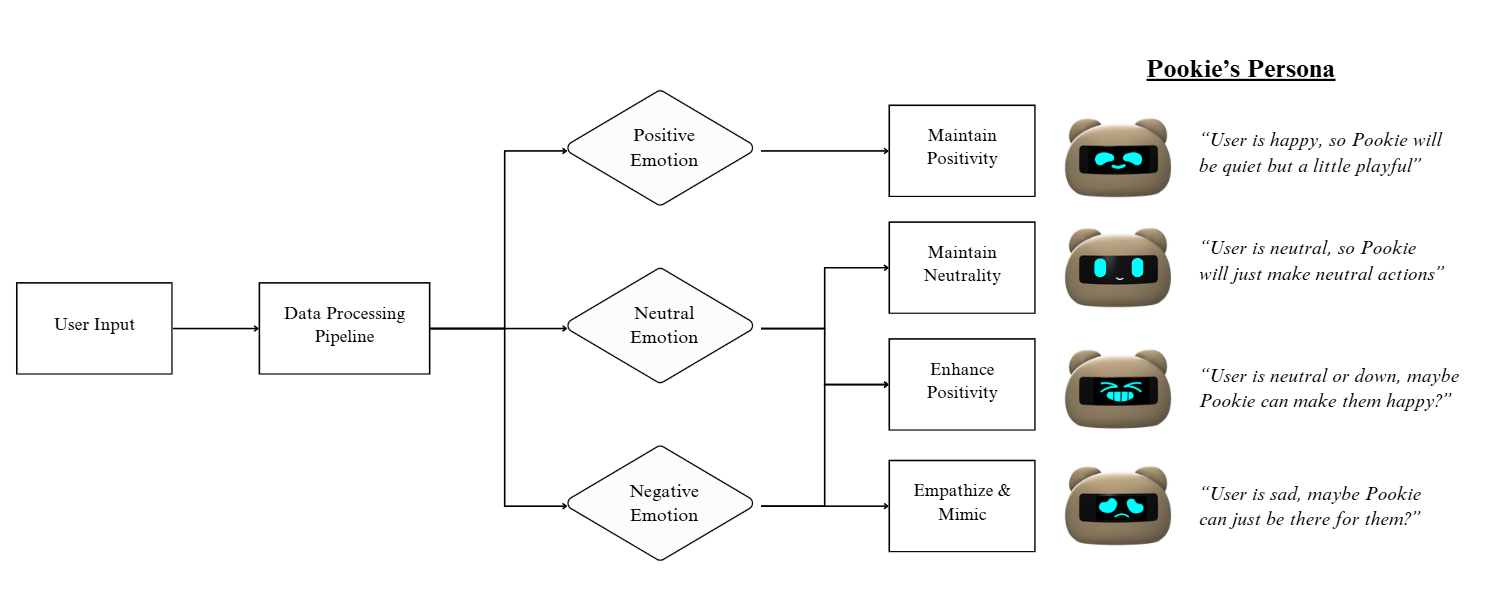
\includegraphics[width=\textwidth]{2-flow.png}
    \captionsetup{justification=centering}
    \caption{Pookie Action Flowchart}
    \label{fig:2-flow}
\end{figure}

Pookie brings together a friendly design and smart features to provide emotional support and comfort to users. It recognizes how a person feels by analyzing facial expressions and voice, then responds in a caring or playful way to match their emotional needs. With this foundation in place, the next section will summarize Pookie’s through two development stages: MVP 1 and MVP 2, carried out during the previous and current academic semesters.

\subsection{MVP 1 - Proof of Concept}
The first phase of the project is named “MVP 1 - Proof of Concept” and spanned the first academic semester. The purpose of this phase was to conduct research to validate the project, as well as build necessary foundations for the second phase. Key initiatives included validating the project concept using primary and secondary research methodologies. On the former side, the team spent three weeks conducting expert interviews with professional psychologists from Chula Student Wellness, a platform for free psychological counseling for Chula students. On the latter side, the team consolidated potential technologies to be used for the implementation of the project, such as potential models to be used for facial emotion recognition, and evaluated them under various factors. 

Overall, the phase came out as a success, with key three objectives fulfilled: designing the physical appearance, designing interactive features, and developing accurate emotion detection algorithms. These achievements lay a significant foundation for the rest of the objectives, where the team must continue building the essential components of the robot, and test under real circumstances. 

\subsection{MVP 2 - Functioning Prototype}
The second phase of the project is named “MVP 2 - Functioning Prototype” and spans the second academic semester. The purpose of this phase was to leverage the foundations established in the first phase, to develop and test the rest of the robot’s components. Key initiatives included enhancing the robot’s emotion detection algorithm, software and hardware integration, and user experience enhancement. Firstly, in terms of the emotion algorithm, the team leveraged Bayesian networks and decision trees to enhance the emotion detection logic. Secondly, regarding integration, the team worked on acquiring and building the hardware components of the robot, then integrating them with the software components to obtain a minimum functioning prototype.  Finally, user experience was enhanced through the use of wake-up words and other features to ensure seamlessness. 

However, given the time constraints and problems encountered throughout the project, the team could not achieve one objective: testing. Initially, the team aimed to test the robot through two methods: a controlled functionality test at MI Innovation Labs, and a long in-depth testing with a single user. Thus, the team focused on improving the user experience instead.

\newpage
\section{Project Development}
\subsection{Concept Development}
Over the next 10 years, the National Innovation Agency (NIA) has identified five major societal challenges related to mental health in Thailand. One of these challenges, dubbed “Terror Outbursts,” refers to incidents of violence or unrest fueled by unresolved societal issues. A deeper analysis reveals that stress and anxiety are significant concerns, with Thailand reporting an average stress rating of 7.7, highlighting the urgent need for intervention. While various solutions are available to address stress and anxiety, the team discovered that simply having someone to listen to is one of the most common and effective forms of support. However, there are moments when a person may not be available to offer comfort, which inspired the creation of Pookie.

Pookie draws inspiration from two key case studies: pets and desktop robots. Pets, such as dogs and cats, are often seen as a source of comfort and relaxation for their owners. Pookie’s design aims to emulate this same sense of comfort and relaxation through resemblance of a pet bear. On the other hand, emotional support robots combine sensors and software to interact with users. Pookie references these interactions and engineering, but adds on another key component that many robots lack: empathy.

With this in mind, the design of Pookie must adhere to two key pillars: empathy and interactivity. The user experience (UX) flow was carefully developed within this framework, which will be explored in the next section.

\subsection{User Experience Development}
\label{sec:ux}
To satisfy the key pillars of empathy and interactivity, the team initially developed the UX flow as shown in Figure \ref{fig:3-init}. According to the diagram, the user sets Pookie up in their home or working environment, and Pookie remains on throughout until the user turns it off. While on, Pookie analyzes the user’s facial and speech emotion, then provides an output personalized to each emotional status. This remained the as-is flowchart for the entirety of MVP 1 and half of MVP 2.

\begin{figure}[ht]
    \centering
    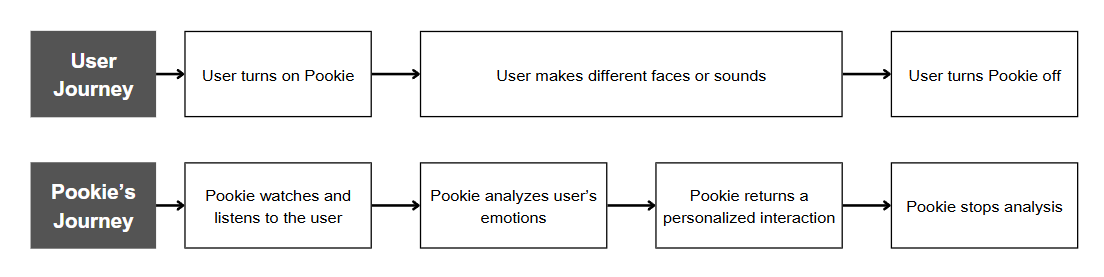
\includegraphics[width=\textwidth]{3-init.png}
    \caption{Initial UX Flowchart}
    \label{fig:3-init} 
\end{figure}

However, upon further empathizing with the user journey, this design lacked the interactivity element. To elaborate, simply having the robot stare at the user for a prolonged amount of time did not seem realistic, and turned out to be a very static design. To address this, the design had to be more dynamic and interactive. The team decided to add an activation layer to the user experience, allowing the user to activate Pookie’s functionalities and turn it off as they please. This was done through the use of \textbf{wake words}, a subset of voice recognition technologies aimed at identifying if a certain word was called out. This new flowchart is shown in Figure \ref{fig:4-revised}.

\begin{figure}[!ht]
    \centering
    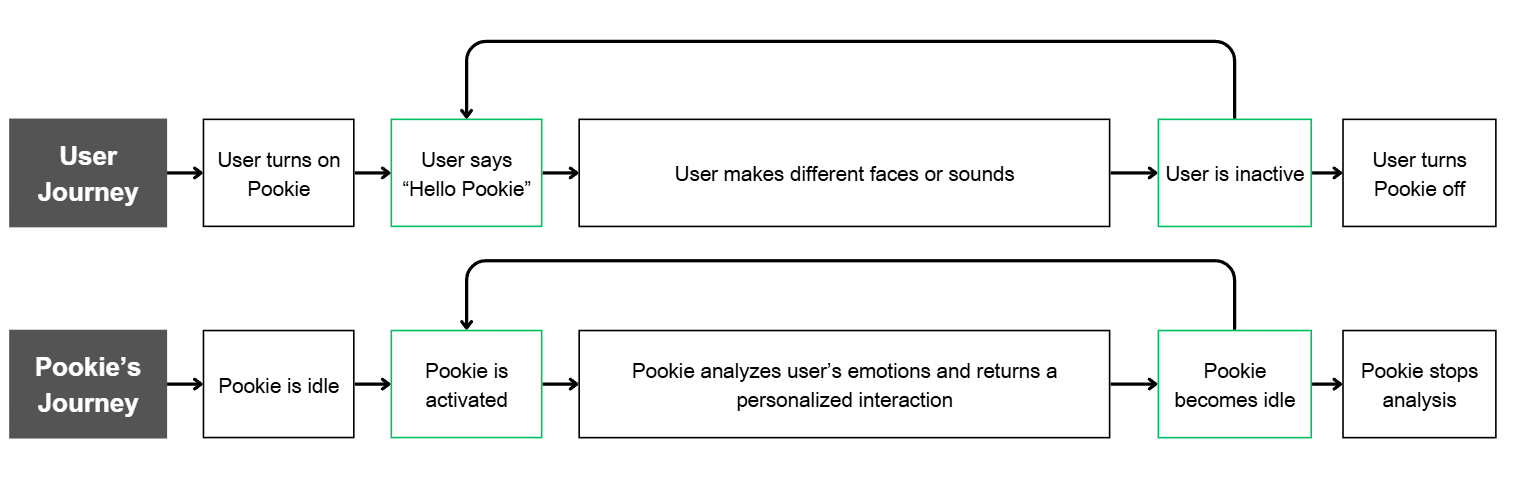
\includegraphics[width=\textwidth]{4-revised.png}
    \caption{Revised UX Flowchart}
    \label{fig:4-revised}
\end{figure}

To achieve this user experience, Pookie must have strong foundations in software and hardware design, being able to accurately determine the user’s emotions and seamlessly carrying out the physical interactions. The software and hardware development initiatives will be discussed in the next sections.

\subsection{Software Development}
In developing the software for Pookie, the tasks were split into 4 layers: activation, classification, decision, and output, as shown in Figure \ref{fig:5-software}. The activation layer represents the wake word “Hello Pookie” detection, which activates the real time input pipeline. Next, the classification layer processes data obtained from the camera and the microphone into the facial and speech emotion recognition models respectively. Moving forward, the decision layer consolidates the emotions detected from the classification layer into a single decision, which determines the output in the output layer. This section will discuss each layer in detail, discussing the rationales behind each technology, results, and challenges.

\begin{figure}[!ht]
    \centering
    \captionsetup{justification=centering}
    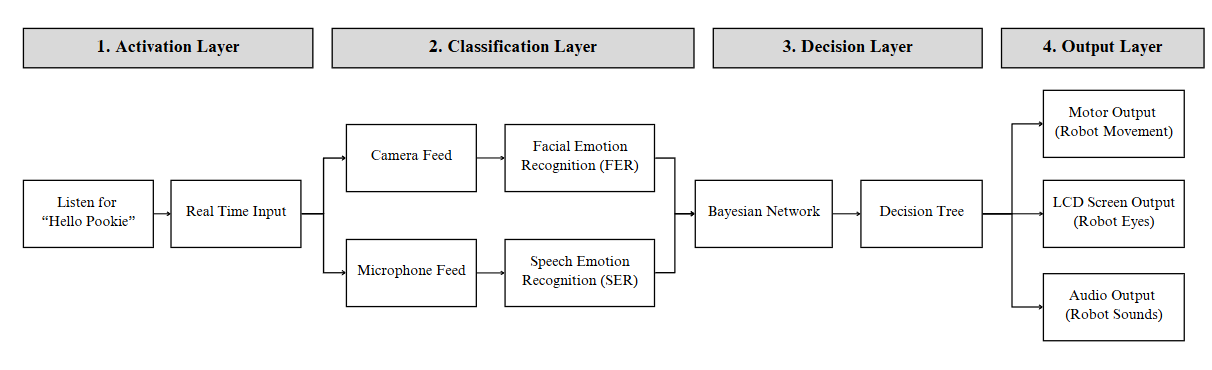
\includegraphics[width=\textwidth]{5-software.png}
    \caption{Software Flowchart}
    \label{fig:5-software}
\end{figure}

\subsubsection{Activation Layer}
The activation layer is primarily responsible for wake word detection—identifying a specific keyword that activates or essentially "wakes up" Pookie. However, developing a precise wake word model from scratch presents numerous challenges and can be a time-consuming process. Given that this was not the central focus of our project, we aimed for a more efficient solution.

Fortunately, Picovoice.ai offers a ready-to-use tool called Porcupine, which enables users to simply input a keyword and generate an offline-compatible model \cite{picovoice_porcupine}. Our team adopted this technology as a rapid and effective addition to the system.

The only challenge we encountered was that Pookie's software was designed to run on the Jetson Orin, which uses an aarch64 architecture and ARM CPU. This caused compatibility issues with some dependencies, especially the Pyporcupine wake word detection library, which is typically tailored for specific hardware platforms. To solve this, we spoofed the Jetson Orin Nano as a Raspberry Pi 5, as both devices run on the same ARM CPU architecture and use the aarch64 instruction set. This allowed us to bypass platform-specific constraints and successfully run Pyporcupine on the Orin.

\subsubsection{Classification Layer}
\label{sec:classification-layer}
The classification layer comprises two essential AI models: the facial and speech emotion recognition models. On one hand, the facial emotion recognition model leverages convolutional neural network (CNN) technologies to learn and extract features from a dataset of faces. On the other hand, the speech emotion recognition model leverages bidirectional long short term memory (LSTMs) to classify speech into respective emotions. It is important to note that the FER model classifies emotions under the seven universal emotions criteria, but the speech emotion recognition model is trained to classify only five. 

In terms of facial emotion recognition, two components must be obtained: the dataset and the model. Regarding the dataset, the facial expression recognition model was trained on a Chinese Faces Dataset , chosen for its similar characteristics to the hard-to-obtain Thai dataset. Utilizing an intuitive approach to synthetic data generation, the dataset was based on a Chinese Face Dataset with Dynamic Expressions and Diverse Ages Synthesized by Deep Learning \cite{han2023}, where a team of researchers created a facial expression image generation model for various Chinese faces belonging to different age groups, genders, and face structure, as shown in Figure \ref{fig:6-face}, labeled as “Ours”. 

\begin{figure}[!ht]
    \centering
    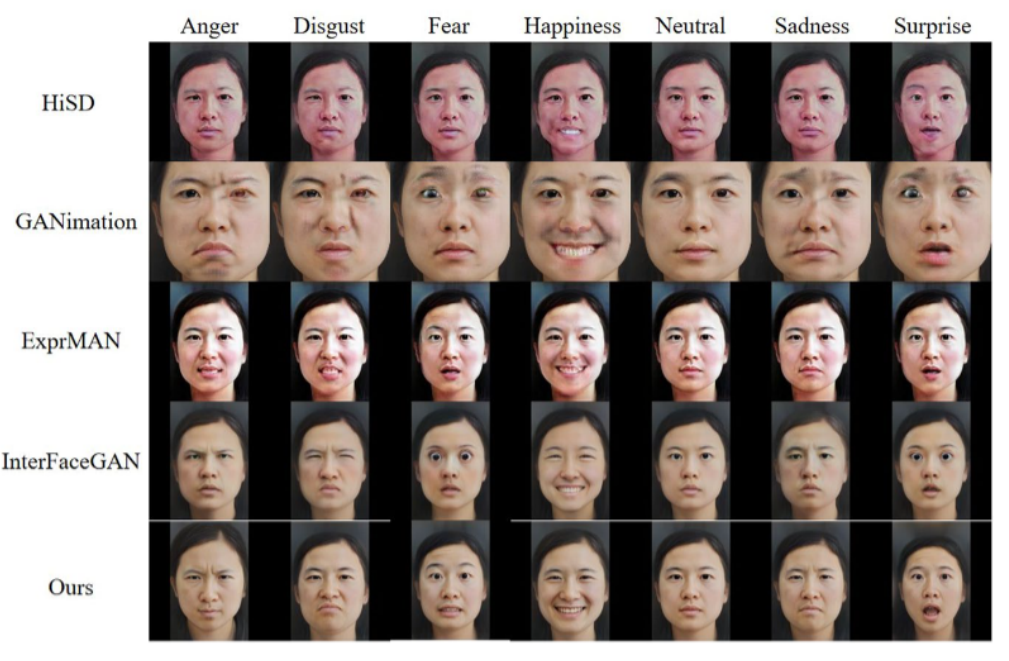
\includegraphics[width=0.8\textwidth]{6-face.png}
    \captionsetup{justification=centering}
    \caption{A Chinese Face Dataset with Dynamic Expressions and Diverse Ages Synthesized. Source: Adapted from \cite{han2023}}
    \label{fig:6-face}
\end{figure}

In terms of model selection, the team utilized three criteria for evaluation: speed, size, and training complexity. Firstly, the model must be fast enough to perform inferences on a real time video feed with minimal latency. Secondly, the size of the model must be lightweight, and highly compatible with the Jetson Orin. Lastly, it must not be too complex to train, with little to no need for additional hyperparameter tuning. 

Upon further analysis, the team singled down on using the VGGNet architecture (Figure \ref{fig:7-vggnet}) —a multi-layer convolutional neural network renowned for feature extraction and classification, particularly in emotion detection models \cite{simonyan2015deepconvolutionalnetworkslargescale}. The decision to select VGGNet was influenced by its balance between performance and implementation simplicity. Although newer architectures like ResNet or EfficientNet offer improved accuracy and deeper representations, they tend to demand more computational resources and training time, which would compromise the low-latency requirement of the system. VGGNet, on the other hand, provides a straightforward layer structure that is easier to deploy on edge devices such as the Jetson Orin, especially when pre-trained weights are utilized.

\begin{figure}[!ht]
    \centering
    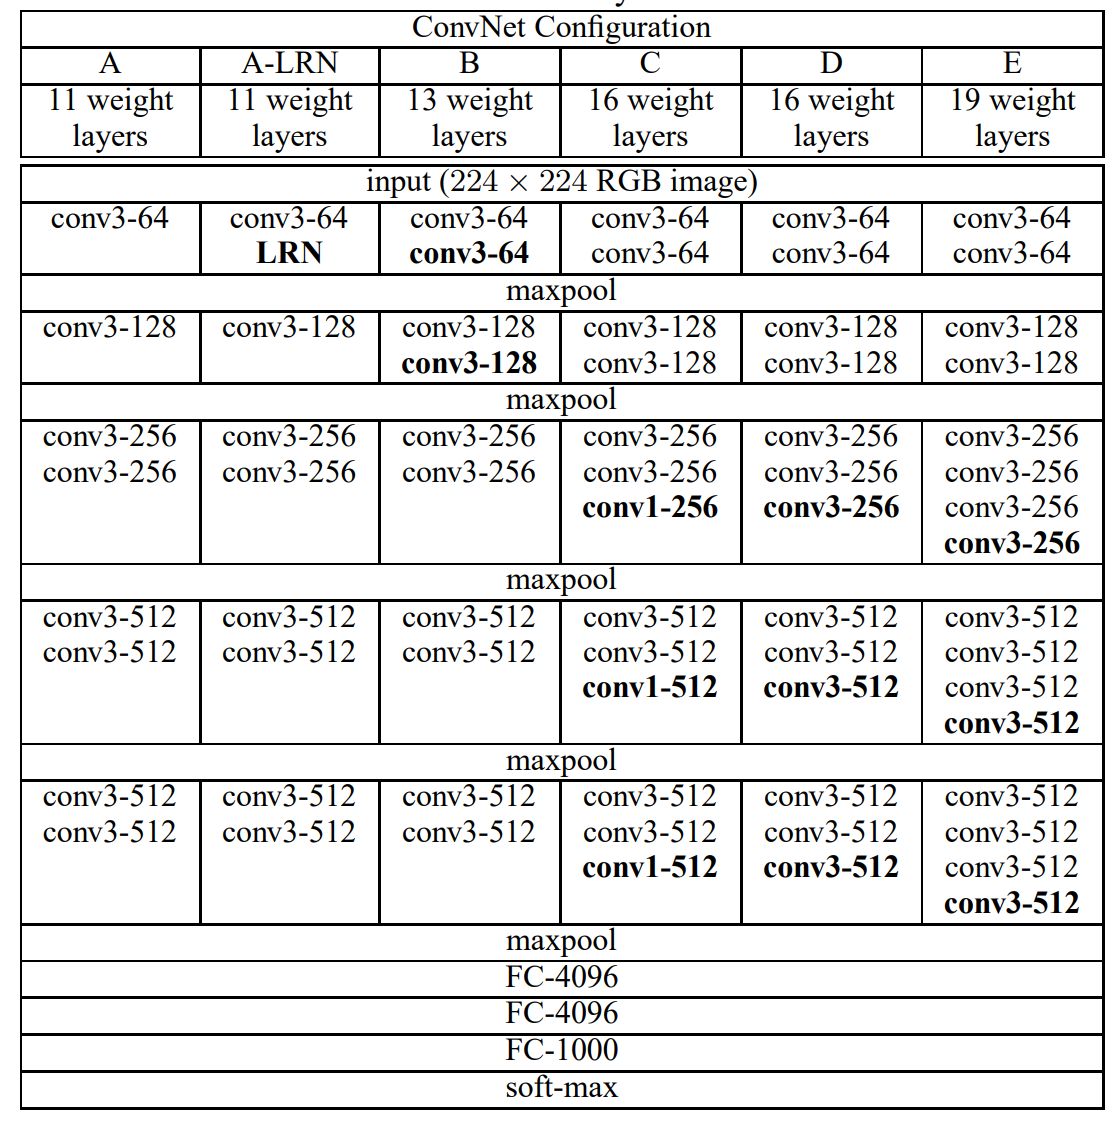
\includegraphics[width=0.75\textwidth]{7-vggnet.png}
    \captionsetup{justification=centering}
    \caption{VGGNet Architecture. Source: Adapted from \cite{simonyan2015deepconvolutionalnetworkslargescale}}
    \label{fig:7-vggnet}
\end{figure}

Thus, the team trained the VGGNet architecture from scratch using the dataset of Chinese faces discussed earlier. Overall, the training results were better than expected, as shown in Table \ref{tab:8-test}, where the model is great at distinguishing between positive emotions such as happiness or surprise, but it is quite lacking in negative emotions. However, given the scope of the project, where positive and neutral are associated with specific outputs, and negative emotions are generally classified as stress, then the model is generally enough to use as a minimum viable product.

\begin{table} [!ht]
    \centering
    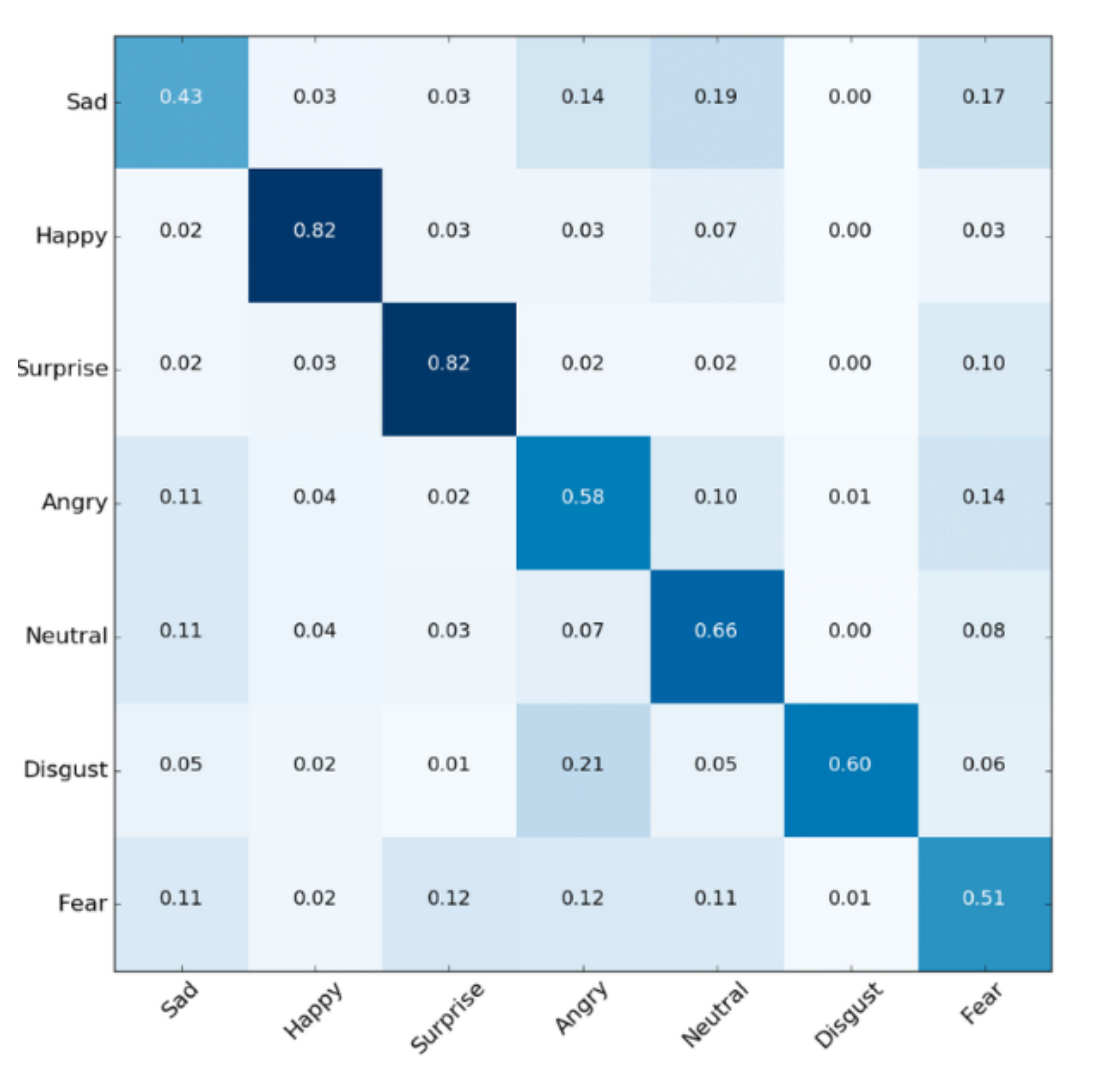
\includegraphics[width=0.7\textwidth]{8-test.png}
    \captionsetup{justification=centering}
    \caption{VGGNet Model Evaluation (Testing Set)}
    \label{tab:8-test}
\end{table}

\newpage
On the other hand, in terms of the speech emotion recognition dataset, the team leveraged a recently published open source Thai Speech Emotion Dataset from VISTEC-depa Thailand AI Research Institute \cite{vistec_ai_ser}, which provides an open source dataset of studio recorded voices with five labels: neutral, anger, happiness, sadness, frustration. The dataset comprises 41 hours and 27,854 sentences of studio recorded voices, with over 200 studio actors. To train this model, VISTEC-depa also utilized a Convolutional Neural Network-Bidirectional Long Short-Term Memory (CNN-BiLSTM) architecture, as shown in Figure \ref{fig:9-lstm}. speech for emotion classification through four stages: converting audio to mel-scale spectrograms, extracting features with 1D CNN and LeakyReLU, capturing temporal patterns via Bidirectional LSTM, and classifying emotions through a Softmax layer. Trained on the VISTEC-depa Thai Speech Emotion Dataset (41 hours, 27,854 sentences from 200+ actors), this hybrid model effectively recognizes five emotions (neutral, anger, happiness, sadness, frustration) by combining CNN's spatial feature extraction with BiLSTM's sequential processing capabilities.

\begin{figure} [!ht]
    \centering
    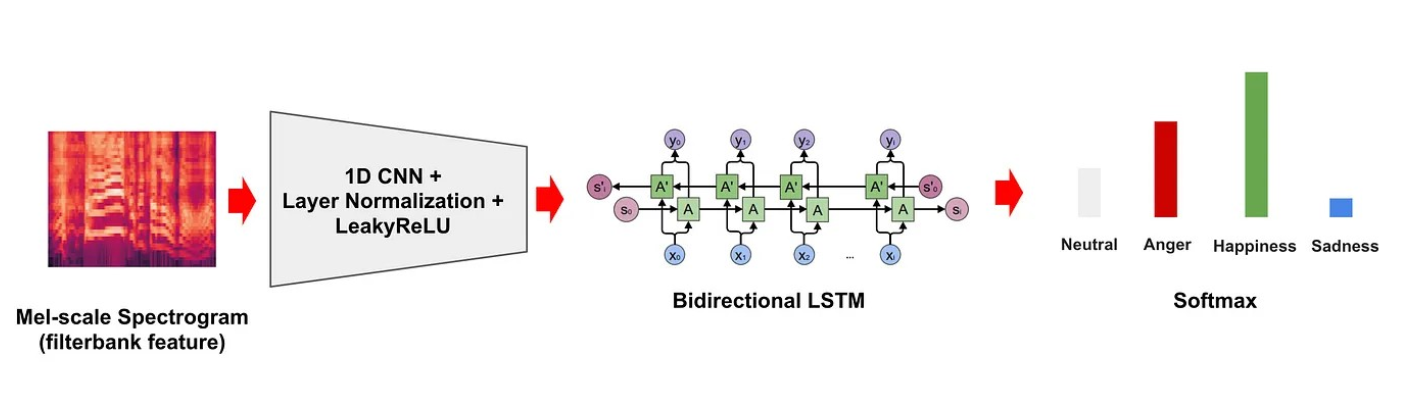
\includegraphics[width=\textwidth]{9-lstm.png}
    \captionsetup{justification=centering}
    \caption{CNN-LSTM Architecture. Source: Adapted from \cite{vistec_ai_ser}}
    \label{fig:9-lstm}
\end{figure}

In terms of evaluation, the CNN-BiLSTM model demonstrated solid performance across all emotional categories, with particularly strong accuracy in identifying neutral speech patterns. Notably, this represents one of the few publicly available Thai speech emotion recognition systems in existence. Given these strengths, the development team integrated this architecture into Pookie for real-time emotion inference capabilities, enabling dynamic emotional assessment during live interactions.

\begin{table} [!ht]
    \centering
    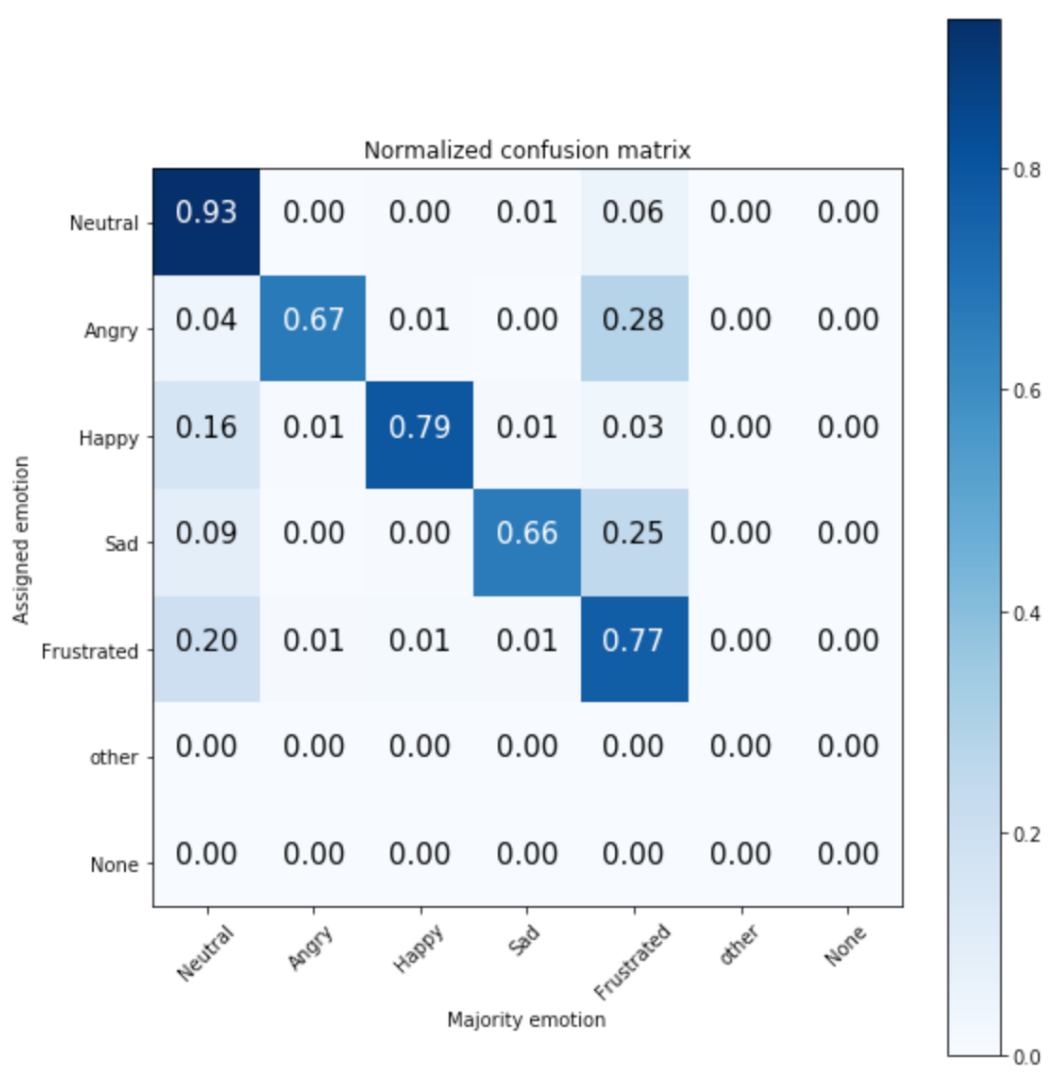
\includegraphics[width=0.7\textwidth]{10-ser.png}
    \captionsetup{justification=centering}
    \caption{SER Model Evaluation. Source: Adapted from \cite{vistec_ai_ser}}
    \label{tab:10-ser}
\end{table}

\subsubsection{Decision Layer}
While Pookie can now successfully determine the user’s emotion through their face and speech, it does not answer the main question: what is the user actually feeling? This cannot be answered easily, as the models produce different sets of outputs, leading to potential ambiguity. For context, each of the FER and SER emotions output a JSON of probabilities and their confidence (e.g Happiness 60\%, Neutral 30\%, Anger 10\%), with the potential outputs from each model shown in Table \ref{tab:11-mapping}. As shown in the figure, the models do not produce outputs with a 1:1 relationship, meaning some emotions from FER do not have a SER counterpart (such as FER output “Fear” does not have a corresponding emotion on the SER side).

\begin{table}[h]
    \centering
    \begin{tabular}{|c|c|}
        \hline
        \textbf{Facial Emotion Recognition (FER) Outputs} & \textbf{Speech Emotion Recognition (SER) Outputs} \\
        \hline
        Neutral   & Neutral   \\
        \hline
        Anger     & Anger     \\
        \hline
        Happiness & Happiness \\
        \hline
        Sadness   & Sadness   \\
        \hline
        Disgust   & Frustration \\
        \hline
        Fear      & Sadness (SER)   \\
        \hline
        Surprise  & Neutral (SER)   \\
        \hline
    \end{tabular}
    \caption{Mapping of Emotions for SER and FER}
    \label{tab:11-mapping}
\end{table}

To address this ambiguity, the use of Bayesian networks and decision trees were introduced within the pipeline. The purpose was to consolidate the distributions of emotion recognition confidence from the two models into one source of truth: what the user is theoretically feeling. 

A Bayesian Network is a probabilistic graphical model that represents a set of variables and their conditional dependencies using a directed acyclic graph (DAG). It provides a structured approach to reasoning under uncertainty by encoding the probabilistic relationships between variables. In the context of Pookie, the Bayesian Network is used to infer the user’s true emotional state by integrating evidence from both the FER and SER models. The revised implementation introduces a Bayesian Network shown in Figure \ref{fig:12-bayes}, where the user’s underlying emotional state is treated as a latent variable, which is updated dynamically as new observations from FER and SER arrive. The network consists of nodes representing possible emotions and edges that define the probabilistic dependencies between them. Given an initial prior belief about the user’s emotion, the system updates its belief by incorporating new observations from the FER and SER models using Bayes’ Theorem.

\begin{figure}[!ht]
    \centering
    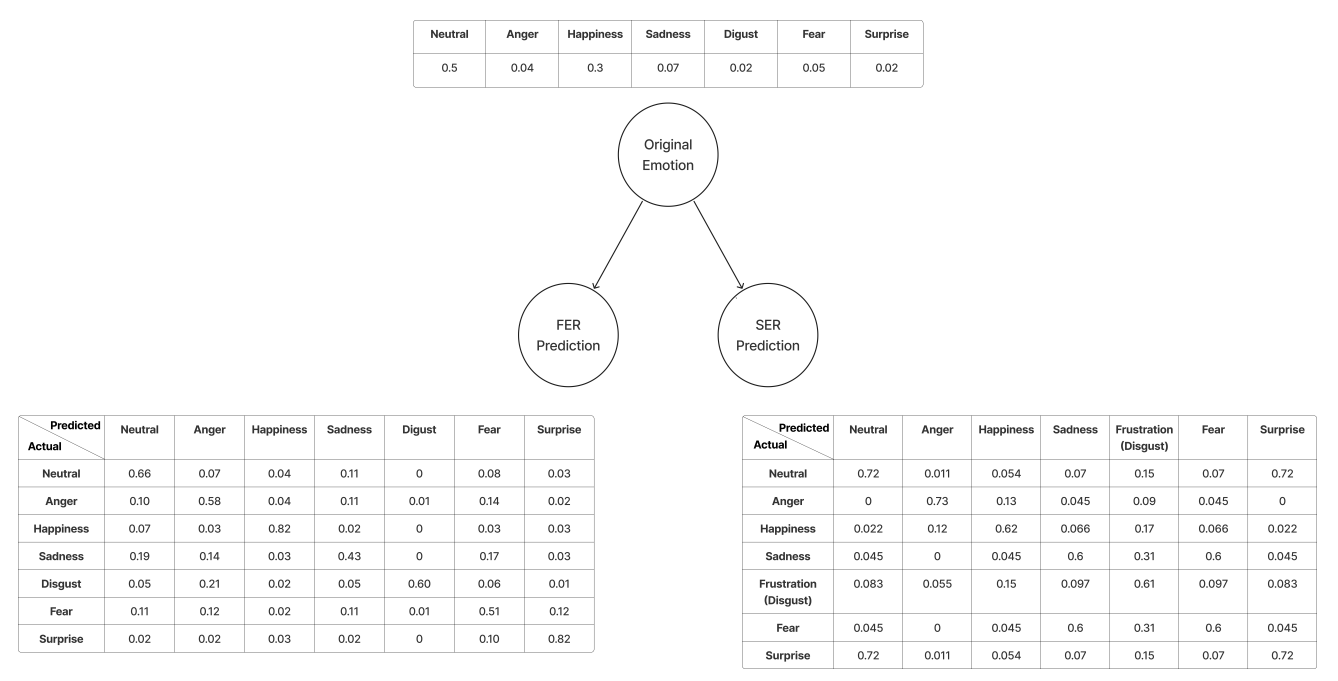
\includegraphics[width=\textwidth]{12-bayes.png}
    \captionsetup{justification=centering}
    \caption{Pookie’s Bayesian Network}
    \label{fig:12-bayes}
\end{figure}

To construct the Bayesian Network, we defined conditional probability tables (CPTs) based on confusion matrices from both the FER and SER models seen in Tables \ref{tab:8-test} and \ref{tab:10-ser} respectively, as well as insights from Emotions in Everyday Life by Trampe et al. (2015) \cite{10.1371/journal.pone.0145450}, which provides probability distributions of emotions. By analyzing the confusion matrices, we estimated the likelihood of misclassifications and incorporated these probabilities into the CPTs, ensuring a more accurate representation of emotional relationships. 

The confusion matrices represent how often the models correctly and incorrectly classify different emotional states. By utilizing these matrices, we were able to estimate the conditional probabilities for each emotional state. For example, if the FER model often misclassifies "Fear" as "Surprise" or "Sadness," these relationships are reflected in the CPTs. Similarly, if the SER model has a tendency to confuse "Frustration" with "Anger," the Bayesian Network accounts for these uncertainties when updating its belief about the user’s true emotion.

By combining the confusion matrix data with the probability distributions from the research paper, we constructed CPTs that better capture real-world emotional correlations. This approach allows the Bayesian Network to weigh the reliability of each model's predictions and adjust the estimated emotional state accordingly. Instead of treating FER and SER outputs as absolute truths, the system considers their likelihood of being correct based on historical performance.

To update the belief about the user’s emotional state, the Bayesian Network relies on Bayes’ Theorem, which provides a framework for calculating conditional probabilities. Specifically, the network uses the formula:

\begin{gather}
    P(E \mid R) = \frac{P(R \mid E) \cdot P(E)}{P(R)}
\end{gather}

Where:
\begin{itemize}
    \item \( P(E \mid R) \) is the posterior probability, representing the probability of the emotional state \( E \) given the result \( R \) (i.e., the FER and SER outputs).
    \item \( P(R \mid E) \) is the likelihood, which indicates how likely the result \( R \) is, given the emotional state \( E \).
    \item \( P(E) \) is the prior probability, representing the initial belief about the emotional state before observing the result, which is informed by the emotion distribution provided in \textit{Emotions in Everyday Life} by Trampe et al. (2015) \cite{10.1371/journal.pone.0145450}.
    \item \( P(R) \) is the evidence, or the total probability of observing the result under all possible emotional states.
\end{itemize}

In the context of Pookie, the emotional state \( E \) could be one of the possible emotions such as happiness, sadness, anger, etc. The result \( R \) is derived from the outputs of the FER and SER models, which provide a set of probabilities for each emotion. The likelihood \( P(R \mid E) \) is determined by the confusion matrices of the FER and SER models, which reflect how likely it is for the models to generate certain outputs given the true emotional state.

In this case, the likelihood \( P(R \mid E) \) is represented as the product of the probabilities from both the Facial Emotion Recognition (FER) and Speech Emotion Recognition (SER) models. Since we are dealing with two different models that provide independent estimates of the user’s emotional state, we combine these estimates by multiplying their corresponding probabilities for each emotion.

Thus, the likelihood for each possible emotional state \( E \) given the result \( R \) (which consists of the outputs from both the FER and SER models) can be expressed as:

\begin{gather}
    P(R \mid E) = P(R_{\text{FER}} \mid E) \cdot P(R_{\text{SER}} \mid E)
\end{gather}


Where:
\begin{itemize}
    \item \( P(R_{\text{FER}} \mid E) \) is the probability of the FER result \( R_{\text{FER}} \) given the emotional state \( E \).
    \item \( P(R_{\text{SER}} \mid E) \) is the probability of the SER result \( R_{\text{SER}} \) given the emotional state \( E \).
\end{itemize}

Since the FER and SER models are independent, their combined likelihood is simply the product of their individual likelihoods. This approach assumes that facial and speech expressions are conditionally independent given the true emotional state. By multiplying the probabilities, we take into account both the visual and auditory evidence of the user’s emotion, and use the combined evidence to estimate the true emotional state more accurately.

Thus, the updated Bayesian formula for computing the posterior probability of the emotional state \( E \) given the observations \( R_{\text{FER}} \) and \( R_{\text{SER}} \) becomes:

\begin{gather}
    P(E \mid R_{\text{FER}}, R_{\text{SER}}) = \frac{P(R_{\text{FER}} \mid E) \cdot P(R_{\text{SER}} \mid E) \cdot P(E)}{P(R_{\text{FER}}, R_{\text{SER}})}
\end{gather}

Where:
\begin{itemize}
    \item \( P(R_{\text{FER}}, R_{\text{SER}}) \) is the evidence or the total probability of observing both the FER and SER results. This is computed as the sum of the likelihoods over all possible emotional states:
\end{itemize}

\begin{gather}
    P(R_{\text{FER}}, R_{\text{SER}}) = \sum_{E} P(R_{\text{FER}} \mid E) \cdot P(R_{\text{SER}} \mid E) \cdot P(E)
\end{gather}

This formulation ensures that the system updates its belief about the user's emotional state by considering the likelihood of both the FER and SER outputs for each possible emotion. By combining the results from the facial and speech emotion recognition models, the Bayesian Network effectively integrates multiple sources of evidence, resulting in a more robust and accurate estimate of the user's true emotional state.

The use of multiplication for the likelihoods allows the Bayesian Network to properly account for the evidence from both modalities, reducing the impact of uncertainties and ambiguities from individual models. This approach improves the overall accuracy of the emotional assessment and enhances the robot's ability to make decisions that align with the user's true feelings.

The prior \( P(E) \) is based on a generalized distribution of emotional states, derived from external research, such as the findings from \cite{10.1371/journal.pone.0145450}. It reflects the average emotional distribution across a population and does not adjust based on an individual user’s history or context. This prior probability serves as a baseline, representing the general likelihood of each emotional state before any new observations from the FER and SER models are made.

Finally, \( P(R) \), the evidence, ensures that the posterior probabilities of all possible emotional states sum to 1. This value can be calculated as the sum of the likelihoods over all possible emotional states:

\begin{gather}
    P(R) = \sum_{E} P(R \mid E) \cdot P(E)
\end{gather}

By applying Bayes’ Theorem iteratively as new observations from the FER and SER models arrive, the Bayesian Network updates its belief about the user's emotional state. This update does not involve refining the estimate based on previous emotional history, but rather adjusts the system’s estimate by integrating the evidence from the two models in real time. This process allows the system to more accurately infer the user’s emotional state and navigate complex emotional situations with greater precision, reducing ambiguity and improving the overall user experience.

This probabilistic model enables Pookie to move beyond simple rule-based decision-making and handle the complexity of real-world emotional states more effectively.

The calculated outputs from the Bayesian network are passed onto a custom decision tree, comprising various nodes containing conditions and actions. The decision tree references the framework shown in Figure \ref{fig:2-framework} to determine the type of action, where the Bayesian network and other data processing pipelines produces an output that is classified into positive, neutral, or negative. With each type of emotion, Pookie then decides whether or not to maintain, enhance, or empathize with the emotion. 

\begin{figure}[ht]
    \centering
    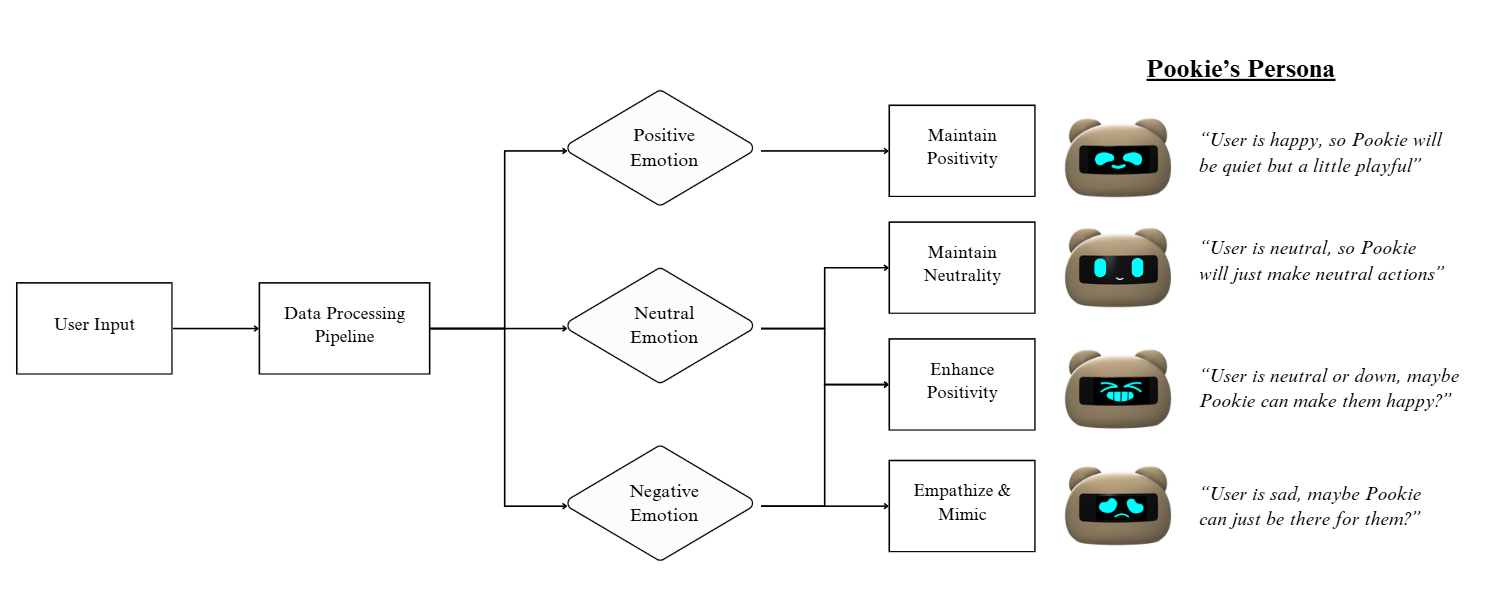
\includegraphics[width=\textwidth]{2-flow.png}
    \captionsetup{justification=centering}
    \caption{Framework for Action Classification}
    \label{fig:2-framework}
\end{figure}

The decision tree consists of 7 branches and a total of 65 nodes with each branch representing a specific dominant emotion. Subsequent layers correspond to conditional checks that help determine the most appropriate action for Pookie to take. An example of such a branch is illustrated in Figure \ref{fig:13-dt}. As shown in the diagram, the initial layer evaluates the output from the Bayesian network to assess whether the dominant emotion is neutral. The following layers then apply additional filters—such as verifying whether positive emotions outweigh negative ones—to further refine the decision. Ultimately, an action is selected based on the emotional state. For example, if the user exhibits predominantly negative emotions, Pookie may respond by making playful eye gestures to uplift the user's mood, an action categorized as “positive enhancement.”

\begin{figure}[ht]
    \centering
    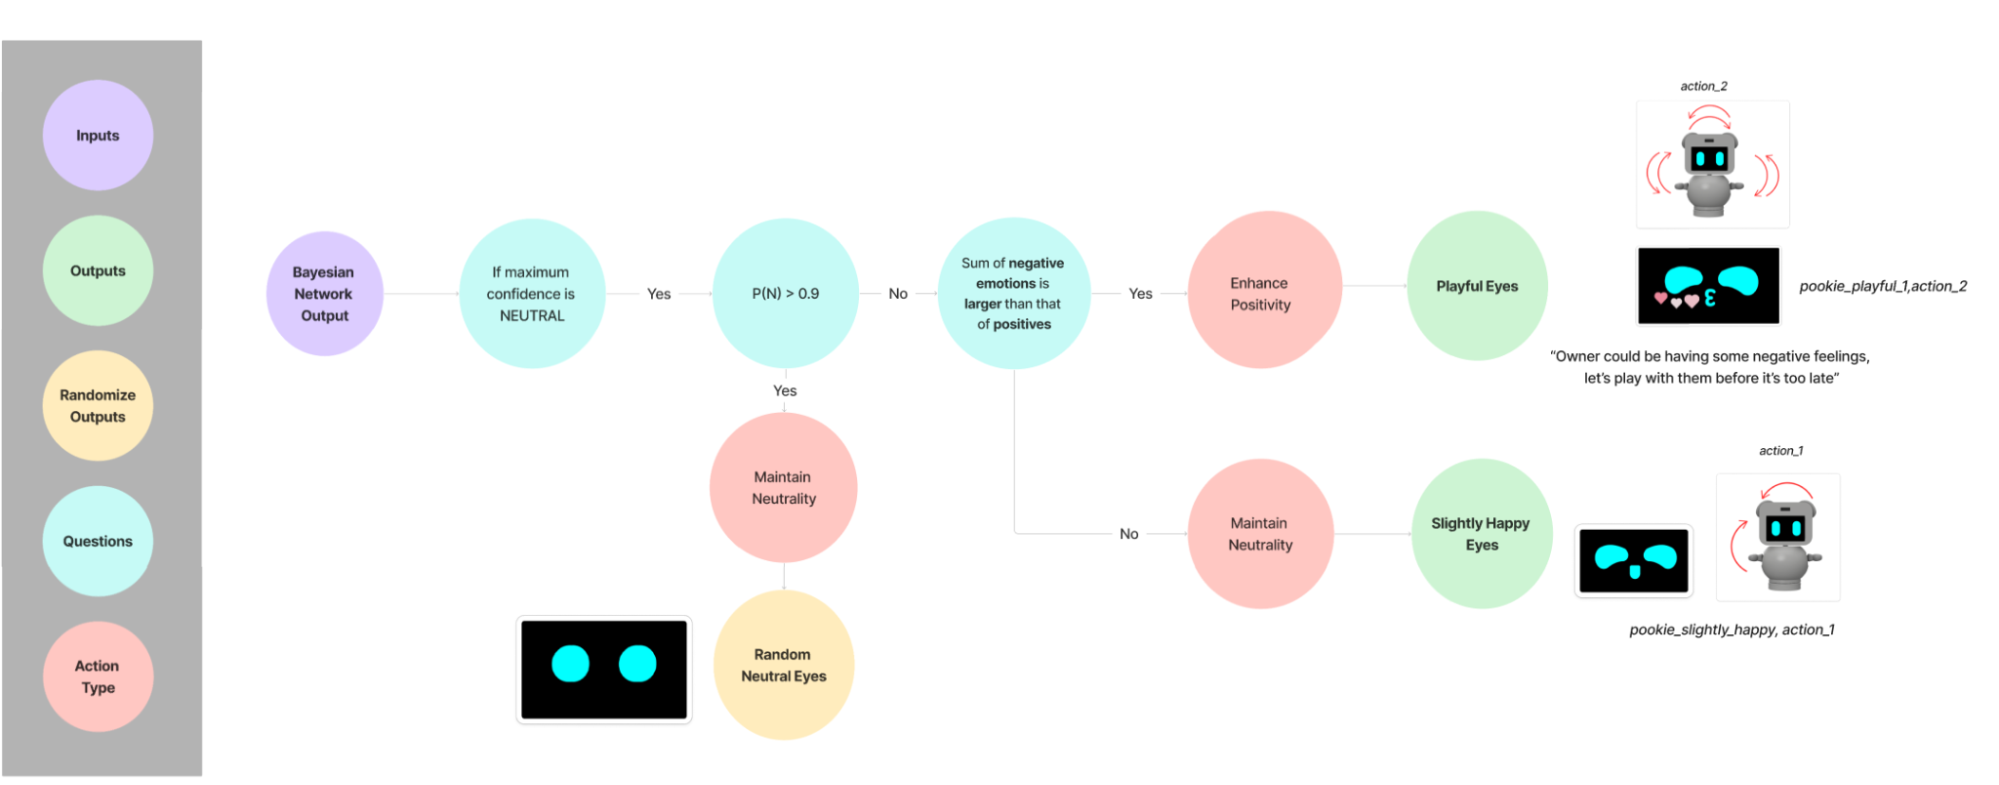
\includegraphics[width=\textwidth]{13-dt.png}
    \captionsetup{justification=centering}
    \caption{Decision Tree Example}
    \label{fig:13-dt}
\end{figure}

\subsubsection{Output Layer}
Finally, the output layer comprises three actions: eye movement, physical movement, and sound. Firstly, the eye patterns are delivered through the LCD Screen as a sequence of frames in a Graphics Interchange Format (GIF). Some examples of eye representations are shown in Figure \ref{fig:14-eye}. These sequences of eye frames were created in Canva, a web application for making powerpoint slides or sequences of images, where the team has built a total of 20 different eye frames to give Pookie another level of interaction.

\begin{figure}[!ht]
    \centering
    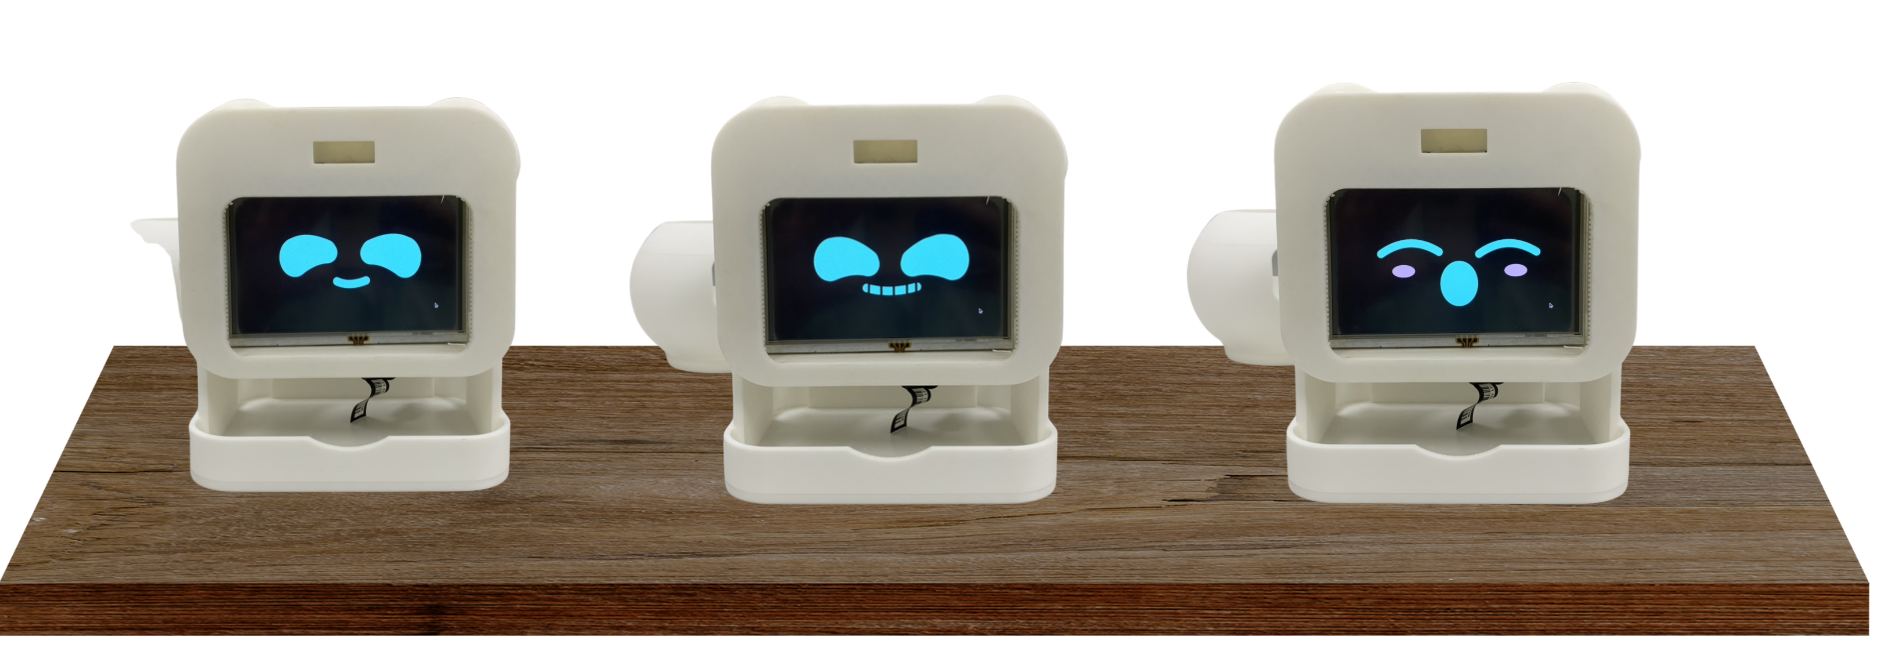
\includegraphics[width=\textwidth]{14-eye.png}
    \captionsetup{justification=centering}
    \caption{Pookie Eye Examples}
    \label{fig:14-eye}
\end{figure}

\newpage
Next, the physical movement patterns were manually programmed to align with the decision tree and framework described in the previous section. Figure \ref{fig:15-move} showcases examples of the movements Pookie is capable of performing. Specifically, Pookie possesses four axes of motion—located at its neck, two arms, and base—which enable it to engage in expressive, interactive behavior with the user.

\begin{figure}[!ht]
    \centering
    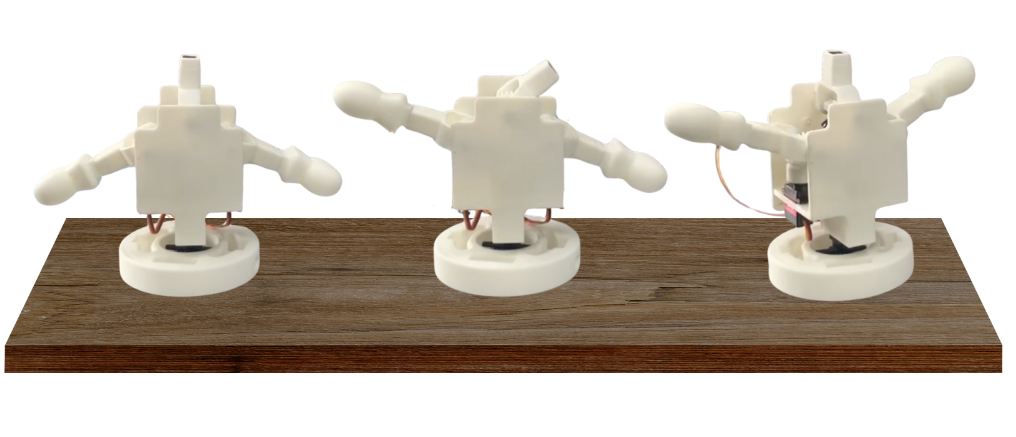
\includegraphics[width=\textwidth]{15-move.png}
    \captionsetup{justification=centering}
    \caption{Pookie Body Movements (Interior)}
    \label{fig:15-move}
\end{figure}

Lastly, sound effects were integrated using an open-source platform called Epidemic Sound, which offers a wide range of royalty-free sound effects for download. These audio elements were selected to complement Pookie’s actions and enhance user interaction.

\subsection{Software Pipeline Evaluation}

\subsubsection{Experiment Overview}
For each output theme, 10 trials were conducted to evaluate the consistency of the emotion pipeline. In each trial, the tester assumed an emotion, after which \textit{Pookie} predicted the emotion and generated a corresponding output. If the assumed emotion and the predicted emotion matched, the trial was labeled as an \textbf{\textit{Intended Result}}.

\newpage
\subsubsection{Remarks}
\begin{itemize}
    \item Results caused by identifiable bugs were excluded. Potential bugs included:
    \begin{itemize}
        \item The robot unexpectedly transitioning to a sleep state.
        \item Asynchronous behavior in the robot's outputs.
    \end{itemize}
    \item The experiment may contain inherent bias:
    \begin{itemize}
        \item Testers were deliberately expressing specific emotions, which does not fully reflect real-world circumstances.
    \end{itemize}
    \item Based on statistical calculations, a total of 246 trials would be required to achieve a 95\% confidence level in the overall evaluation.
\end{itemize}

\subsubsection{Confidence Level Calculation}
To determine the number of trials required for evaluating the emotion pipeline with statistical confidence, we used the following standard formula for estimating sample size in proportion-based accuracy testing:

\[
n = \left(\frac{Z^2 \cdot p\cdot(1 - p)}{E^2}\right)
\]

Where:
\begin{itemize}
    \item \( n \) is the required sample size,
    \item \( Z \) is the z-score corresponding to the desired confidence level,
    \item \( p \) is the estimated accuracy (proportion of intended results),
    \item \( E \) is the acceptable margin of error.
\end{itemize}

For a 95\% confidence level, we use \( Z = 1.96 \). Assuming an estimated accuracy of \( p = 0.80 \), and a margin of error \( E = 0.05 \), the calculation is:

\[
n = \left(\frac{1.96^2 \cdot 0.8 \cdot (1 - 0.8)}{0.05^2}\right)
\approx 246
\]

Thus, approximately 246 trials are needed to evaluate the pipeline with a 95\% confidence level and a ±5\% margin of error.

\subsubsection{Results}
\begin{enumerate}
    \item \textbf{Emotional Maintenance:} \textit{90\%} of trials were successful.
    \begin{table}[!ht]
        \centering
        \resizebox{\textwidth}{!}{
        \begin{tabular}{|c|l|l|l|l|l|}
        \hline
        \textbf{Trials} & \textbf{Forms of Input} & \textbf{Prediction} & \textbf{Assumed Action} & \textbf{Actual Action} & \textbf{Remarks} \\
        \hline
        1 & FER Only (Slight Smile) & Happiness 62.4\% & Slightly Happy / Very Happy & Slightly Happy & Intended Result \\
        \hline
        2 & FER Only (Normal Smile) & Happiness 74.0\% & Slightly Happy / Very Happy & Very Happy & Intended Result \\
        \hline
        3 & FER Only (Exaggerated Smile) & Happiness 82.1\% & Slightly Happy / Very Happy & Slightly Happy & Intended Result \\
        \hline
        4 & FER Only (Surprised Face) & Surprise 64.6\% & Surprise 3 & Surprise 3 & Intended Result \\
        \hline
        5 & FER Only (Resting Face) & Neutral 60.2\% & No action & No action & Intended Result \\
        \hline
        6 & \makecell[l]{Bayesian Network (FER + SER) \\ (Laughing face with laughing voice)} & Happiness & Very Happy & Very Happy & Intended Result \\
        \hline
        7 & \makecell[l]{Bayesian Network (FER + SER) \\ (Smiling face with neutral voice)} & Sadness & Slightly Happy & Sadness 2 & Unintended Result \\
        \hline
        8 & \makecell[l]{Bayesian Network (FER + SER) \\ (Smiling face with neutral voice)} & Happiness & Playful 2 / Playful 3 & Playful 2 & Intended Result \\
        \hline
        9 & \makecell[l]{Bayesian Network (FER + SER) \\ (Smiling face with neutral voice)} & Happiness & Playful 2 / Playful 3 & Playful 2 & Intended Result \\
        \hline
        10 & \makecell[l]{Bayesian Network (FER + SER) \\ (Neutral face and voice)} & Neutral & No action & No action & Intended Result \\
        \hline
        \end{tabular}
        }
    \caption{Emotion Pipeline Evaluation Trials for Emotional Maintenance}
    \label{tab:14-maintenance} 
    \end{table}
\newpage
    \item \textbf{Positive Enhancement:} \textit{70\%} of trials were successful.
    \begin{table}[!ht]
        \centering
        \resizebox{\textwidth}{!}{
        \begin{tabular}{|c|l|l|l|l|l|}
        \hline
        \textbf{Trials} & \textbf{Forms of Input} & \textbf{Prediction} & \textbf{Assumed Action} & \textbf{Actual Action} & \textbf{Remarks} \\
        \hline
        1 & \makecell[l]{Bayesian Network (FER + SER) \\ (Neutral face with neutral voice)} & Neutral & No Action & No Action & Intended Result \\
        \hline
        2 & \makecell[l]{Bayesian Network (FER + SER) \\ (Sad face with neutral voice)} & Sadness & No Action & Listen 2 & \makecell[l]{Unintended Result} \\
        \hline
        3 & \makecell[l]{Bayesian Network (FER + SER) \\ (Sad face with neutral voice)} & Sadness & No Action & No Action & Intended Result \\
        \hline
        4 & \makecell[l]{Bayesian Network (FER + SER) \\ (Disgusted face with neutral voice)} & Sadness & Listen 5 & Sad 2 & \makecell[l]{Unintended Result} \\
        \hline
        5 & \makecell[l]{Bayesian Network (FER + SER) \\ (Disgusted face with neutral voice)} & Disgust & Listen 5 & Listen 5 & Intended Result \\
        \hline
        6 & \makecell[l]{Bayesian Network (FER + SER) \\ (Disgusted face with sad voice)} & Disgust & Listen 6 & Listen 6 & Intended Result \\
        \hline
        7 & \makecell[l]{Bayesian Network (FER + SER) \\ (Angry face with neutral voice)} & Neutral & No Action & No Action & Intended Result \\
        \hline
        8 & \makecell[l]{Bayesian Network (FER + SER) \\ (Angry face with sad voice)} & Sadness & Listen 2 & Listen 2 & Intended Result \\
        \hline
        9 & \makecell[l]{Bayesian Network (FER + SER) \\ (Surprise face with sad voice)} & Fear & No Action & Surprise 2 & \makecell[l]{Unintended Result} \\
        \hline
        10 & \makecell[l]{Bayesian Network (FER + SER) \\ (Surprise face with sad voice)} & Fear & Surprise 2 & Surprise 2 & Intended Result \\
        \hline
        \end{tabular}
        }
    \caption{Emotion Pipeline Evaluation Trials for Positive Enhancement}
    \label{tab:14-enhancement}
    \end{table}

    \item \textbf{Empathy and Mimicry:} \textit{60\%} of trials were successful.
    \begin{table}[!ht]
        \centering
        \resizebox{\textwidth}{!}{
        \begin{tabular}{|c|l|l|l|l|l|}
        \hline
        \textbf{Trials} & \textbf{Forms of Input} & \textbf{Prediction} & \textbf{Assumed Action} & \textbf{Actual Action} & \textbf{Remarks} \\
        \hline
        1 & FER Only (Frown) & Sadness 60.4\% & Listen 2 & Listen 2 & Intended Result \\
        \hline
        2 & FER Only (Frown) & Sadness 64.0\% & Listen 2 & Listen 2 & Intended Result \\
        \hline
        3 & FER Only (Disgusted) & Disgust 68.5\% & Listen 7 & Listen 7 & Intended Result \\
        \hline
        4 & FER Only (Knitted brow and frown) & Anger 61.7\% & Listen 1 & Listen 1 & Intended Result \\
        \hline
        5 & \makecell[l]{Bayesian Network (FER + SER) \\ (Sad face with sad voice)} & Sadness & Sad 2 & Sad 2 & Intended Result \\
        \hline
        6 & \makecell[l]{Bayesian Network (FER + SER) \\ (Sad face with sad voice)} & Sadness & Listen 2 & Listen 2 & Intended Result \\
        \hline
        7 & \makecell[l]{Bayesian Network (FER + SER) \\ (Angry face with frustrated voice)} & Sadness & Listen 3 & Sad 2 & \makecell[l]{Unintended Result} \\
        \hline
        8 & \makecell[l]{Bayesian Network (FER + SER) \\ (Disgusted face with sad voice)} & Neutral & Listen 6 & No Action & \makecell[l]{Unintended Result} \\
        \hline
        9 & \makecell[l]{Bayesian Network (FER + SER) \\ (Neutral face with sad voice)} & Neutral & Sad 1 & No Action & \makecell[l]{Unintended Result} \\
        \hline
        10 & \makecell[l]{Bayesian Network (FER + SER) \\ (Neutral face with neutral voice)} & Sadness & No Action & Sadness 2 & \makecell[l]{Unintended Result} \\
        \hline
        \end{tabular}
        }
    \caption{Emotion Pipeline Evaluation Trials for Empathy and Mimicry}
    \label{tab:14-empathy} 
    \end{table}
\end{enumerate}

The evaluation of the emotion pipeline across the three behavioral dimensions—\textbf{Emotional Maintenance}, \textbf{Positive Enhancement}, and \textbf{Empathy and Mimicry}—demonstrates a clear trend: the system performs more reliably when interpreting and responding to positive emotional stimuli than to negative ones. Emotional Maintenance trials yielded a \textit{90\%} success rate, with consistent responses to facial expressions associated with happiness and surprise. Similarly, Positive Enhancement achieved a \textit{70\%} success rate, indicating moderate proficiency in sustaining or boosting emotional states, especially when processing neutral or slightly negative cues.

In contrast, the Empathy and Mimicry trials showed only a \textit{60\%} success rate, with several unintended results emerging from inputs involving complex or mixed negative emotions such as sadness, anger, and disgust. These findings suggest that while the system is relatively robust in recognizing and maintaining positive affect, it struggles with accurately interpreting and mimicking nuanced or overlapping negative emotional states—particularly when integrating multimodal inputs from both facial expression recognition (FER) and speech emotion recognition (SER).

It is important to note that due to time constraints, each behavioral condition was evaluated using only \textit{10 trials}. While these preliminary findings offer valuable insights, they are not statistically conclusive. To achieve a statistically significant evaluation with \textbf{95\% confidence}, \textbf{80\% expected accuracy}, and a \textbf{5\% margin of error}, approximately \textit{246 trials per condition} would be required. Future work should prioritize conducting a larger number of trials and enhancing the system’s responsiveness to complex negative emotions to support more nuanced and empathetic human-robot interaction.

\subsection{Hardware Development}
In this section, key hardware components and mechanical system design that enable Pookie to function as an interactive emotional support robot will be discussed. This includes the selection and integration of sensors, actuators, processing units, and supporting electronics, as well as mechanical system design that work together to bring Pookie’s capabilities to life. A well-designed hardware system is fundamental to ensuring responsive, reliable, and emotionally engaging behavior.

\subsubsection{Hardware Components}
To ensure the success of Pookie, a well-integrated combination of hardware components is essential. First, Pookie relies on two primary sensors: video and audio, using a webcam and a microphone to perceive its surroundings. Next, various actuators are needed to produce outputs, including LCD screens to display expressive eyes, motors to enable movement, and sound actuators to deliver audio responses. At the core of Pookie’s functionality is its processing unit, which connects software with hardware. The Jetson Orin microprocessor was chosen for its high performance and efficiency. Finally, supporting electrical components such as motor drivers and batteries provide the power and control required to maintain smooth and reliable operation throughout the system.

\begin{table}[h]
    \begin{center}
    \begin{tabular}{|c|c|}
        \hline
        \textbf{Components} & \textbf{Purpose} \\
        \hline
        5 Inches TFT Touch Screen For RPI3 and RPI4B & Pookie’s visual interface (eye)   \\
        \hline
        Logitech Brio 100 Full HD 1080p Webcam     & Pookie’s camera     \\
        \hline
        Jetson Audio CODEC & Enables audio input/output (Pookie’s microphone, sound) \\
        \hline
        TD-8125MG Digital Servo 25kg   & Facilitates head movement   \\
        \hline
        MG90S Servo Metal Gear Tower Pro   & Facilitates arm and body movement \\
        \hline
        Adafruit PCA9685 Servo Driver      &  Communicates between Orin and the servo motors   \\
        \hline
        12V 6Ah Battery  & Powers the motors connected to the driver   \\
        \hline
        51105 SKF Thrust Bearing &  Supports the overall mechanical load of the body \\
        \hline
        Jetson Orin 8GB &  Main processing unit for Pookie, connects all components \\
        \hline
    \end{tabular}
    \end{center}
    \captionsetup{justification=centering}
    \caption{Pookie’s Hardware Components and Purpose}
    \label{tab:16-hardware}
\end{table}

\subsubsection{Mechanical System Design}
Pookie comprises four degrees of freedom, all in the form of revolute joints. The purpose of these joints are to drive movement in the head, arms, and base of the robot. Figure \ref{fig:16-interior} illustrates the interior components of the robot. As shown, it comprises a series of motors, gears, shafts, and bearings. All of these components work together to deliver the physical actions conceptualized in the previous sections. 

\begin{figure}[!ht]
    \centering
    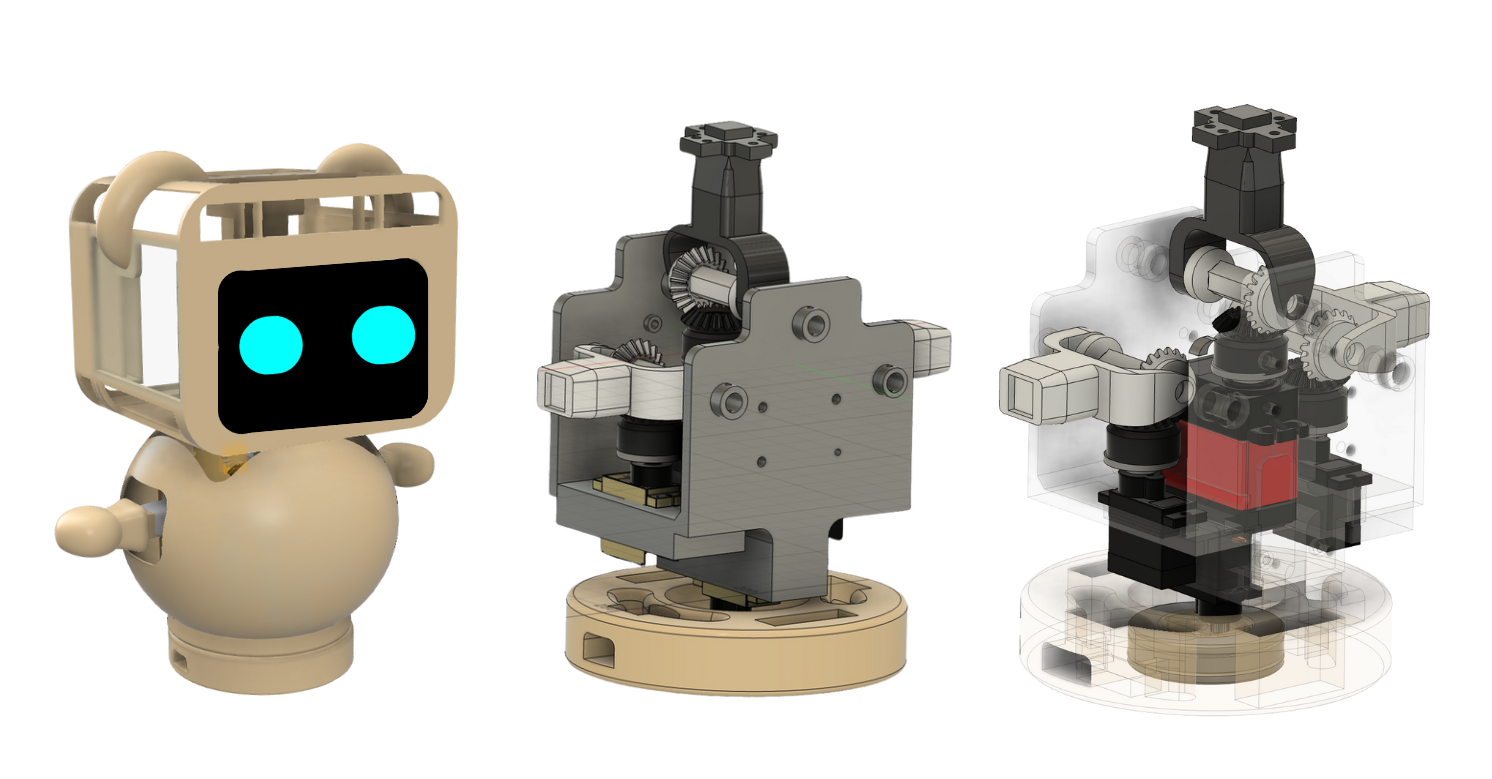
\includegraphics[width=\textwidth]{16-interior.png}
    \captionsetup{justification=centering}
    \caption{Interior Components of Pookie}
    \label{fig:16-interior}
\end{figure}

To enhance design efficiency and modularity, all motors are strategically positioned on a common plane, driving rotational motion along the z-axis. This layout not only simplifies the mechanical structure but also facilitates easier maintenance and part replacement. As shown in Figure \ref{fig:17-kinematics}, a bevel gear system is employed to transfer motion across axes, allowing Pookie to perform complex movements despite having its actuators located in a single plane. This approach optimizes space usage while maintaining full functionality across multiple degrees of freedom. 

\begin{figure}[!ht]
    \centering
    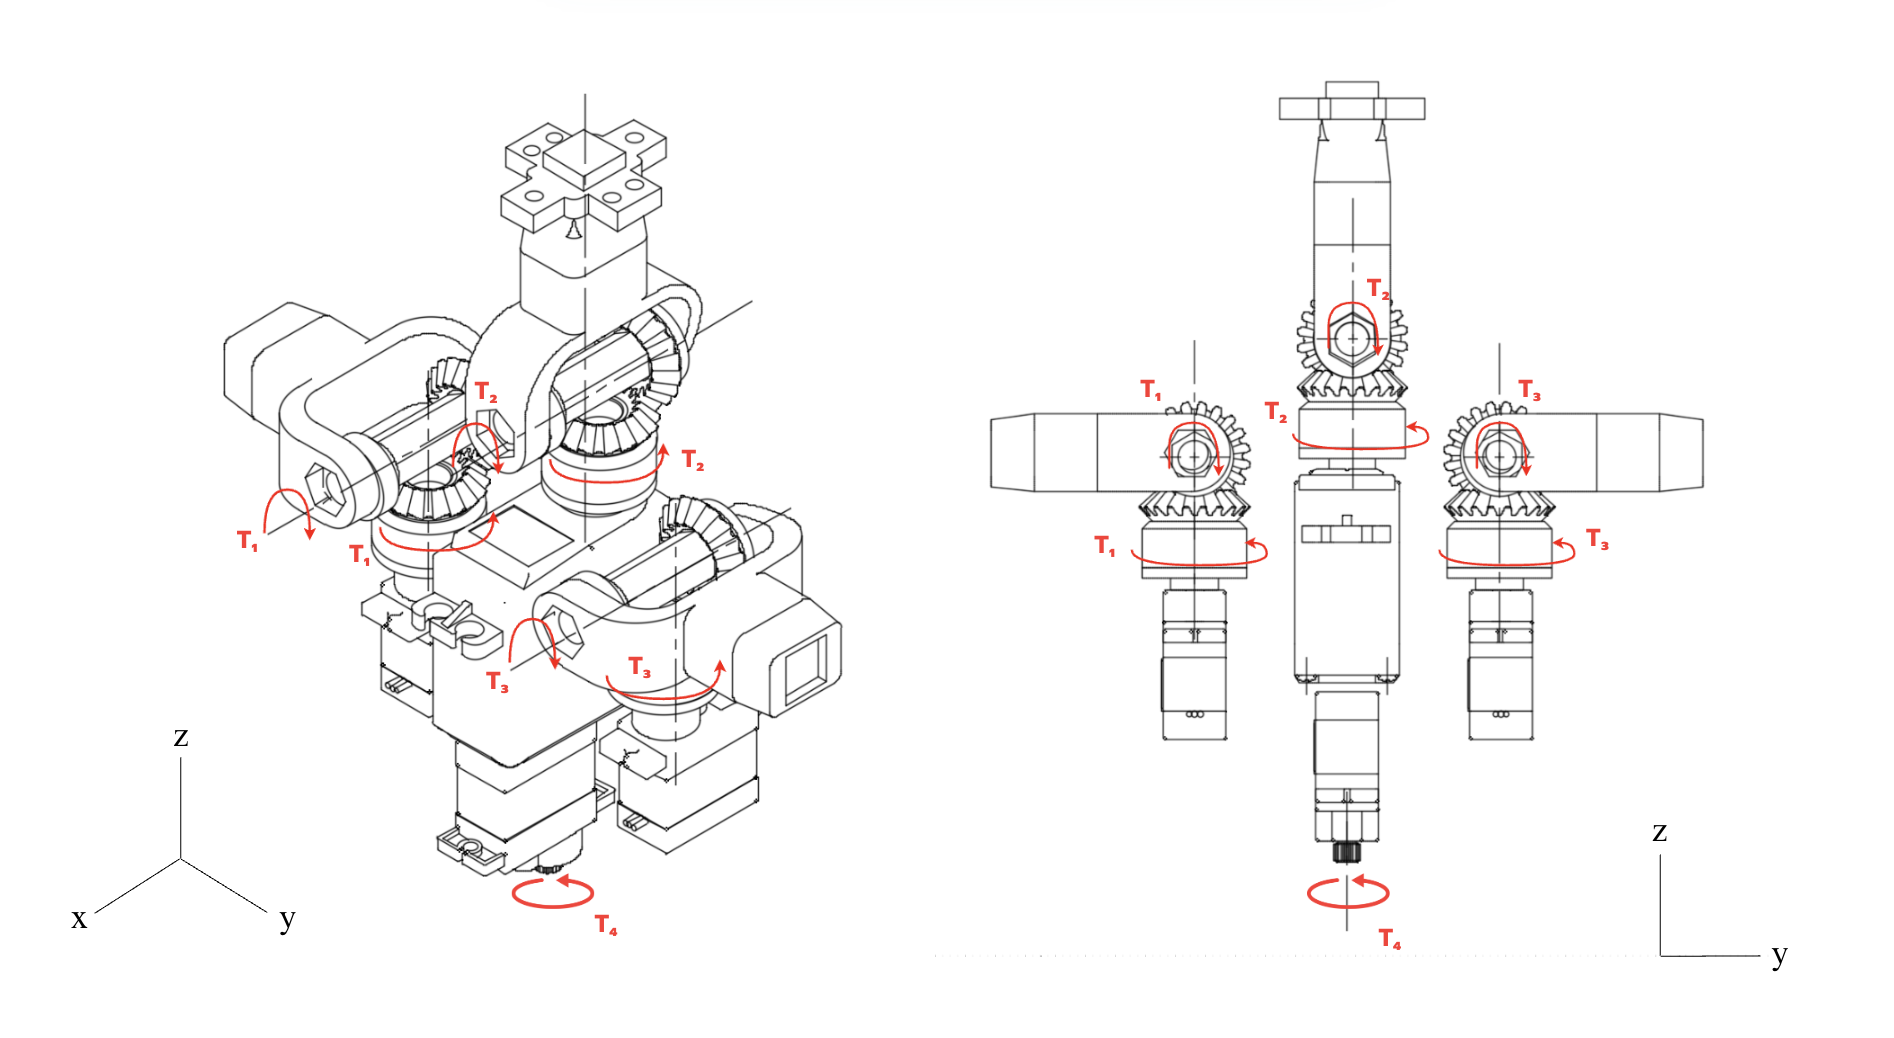
\includegraphics[width=\textwidth]{17-kinematics.png}
    \captionsetup{justification=centering}
    \caption{Pookie Kinematics}
    \label{fig:17-kinematics}
\end{figure}

The bevel gear system is all equal in the number of gear teeth (n). Thus, according to the governing equation for gear ratios shown below, an equal amount of gear teeth constitutes a 1:1 transmission in torque (T). This rule holds true if Pookie comprises a rigid body. 

\begin{gather}
    \frac{n_1}{n_2} = \frac{T_2}{T_1}
\end{gather}

Given this design, two mechanical concerns arise: the torque required to move the head and the load on the base. For torque, Pookie’s arms are lightweight, composed only of a hollow 3D-printed hand and a few embedded magnets. This minimal mass requires very little torque, making the MG90S motor—with a torque rating of 0.18 to 0.22 N·m—an appropriate choice.

In contrast, Pookie’s head contains multiple heavier components, including the LCD screen, wiring adapters, and structural elements, which place a significantly greater torque demand on the motor. While the arms may require less than 0.2 N·m of torque to operate, the head demands over 0.8773 N·m just to remain stable under static conditions. To accommodate this, the TD-8125MG digital servo was selected, delivering a holding torque of 2.31 to 2.63 N·m, which provides a robust safety margin at approximately three times the necessary torque.

The second concern is the vertical load placed on the base motor, responsible for rotating the robot along the z-axis. This motor supports a vertical load exceeding 10 N, resulting from the combined weight of the robot’s upper body and mechanical components. Relying solely on the motor shaft for this axial load would risk rapid wear or mechanical failure. To address this, thrust ball bearings were integrated into the base assembly. Specifically, the team leveraged a 51105 Single direction thrust ball bearing, as there is no radial load on the base.

\begin{figure}[!ht]
    \centering
    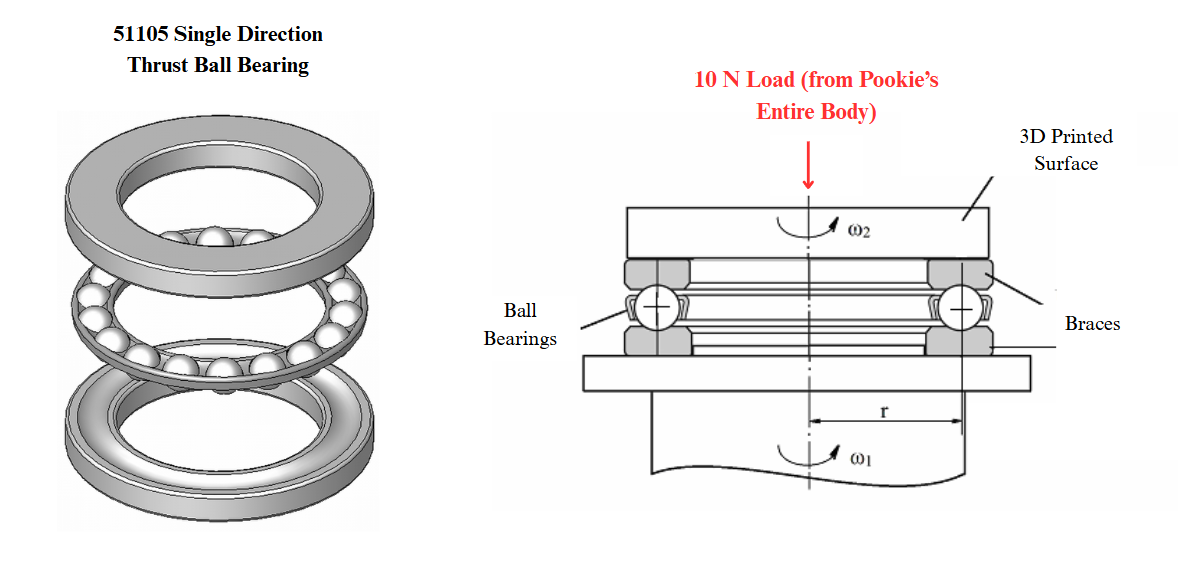
\includegraphics[width=\textwidth]{18-bearings.png}
    \captionsetup{justification=centering}
    \caption{Thrust Ball Bearing. Source: Adapted from \cite{Olaru_2016}}
    \label{fig:18-bearings}
\end{figure}

These specialized bearings are designed to handle high axial loads efficiently, transferring vertical forces away from the motor shaft and distributing them across a broader surface. This ensures smoother rotation, reduces friction, and significantly extends the motor’s operational lifespan.


\newpage
\section{Testing Methodology}
\label{sec:testing-methodology}
This section proposes the methodology for end-user testing, designed to evaluate Pookie’s ability to recognize human emotions and deliver responses that promote emotional well-being—specifically by reducing anxiety and encouraging a positive mental state. Although the team initially planned to conduct these tests within the current semester, unforeseen time constraints prevented the completion of user trials.

The testing will take place in a controlled setting at the MI Innovation Labs, located in the 100th Year Engineering Building, over a period of 1 to 2 weeks. During this period, students will be invited to interact with Pookie and provide feedback on their experience. The MI Labs were selected due to their consistent foot traffic from our target demographic—users aged 18 and above—and their safe, enclosed environment conducive to focused interaction. A team member will be present at all times to supervise the sessions and administer pre- and post-interaction surveys, which will capture shifts in users' self-reported anxiety and positivity levels.

While this setup allows for a higher volume of interactions and supports more robust data analysis, it does not fully simulate Pookie’s envisioned integration into users’ daily routines.  One limitation of this approach is the testing location itself: the MI Innovation Labs primarily attract engineering students, which could lead to sampling bias. Nonetheless, as the target population includes individuals aged 18 and above with mild to moderate anxiety, engineering students still represent a reasonably valid subset of this broader demographic.

Each user interaction will last approximately five minutes, excluding time allocated for briefing and debriefing. A detailed breakdown of the experimental parameters is provided in Table \ref{tab:19-experiment}.

\begin{table}[h]
    \centering
    \begin{tabular}{|c|c|}
        \hline
        \textbf{Parameter} & \textbf{Detail} \\
        \hline
        Format   & Quantitative Questionnaire; Total 10 Questions   \\
        \hline
        Environment     & MI Innovation Labs, 100th Year Building, M Floor     \\
        \hline
        Experiment Time & Approximately 5 minutes per person     \\
        \hline
        Target Segment & Students aged 18 and above     \\
        \hline
    \end{tabular}
    \caption{Experiment Parameters}
    \label{tab:19-experiment}
\end{table}

As previously mentioned, users will be asked a series of questions before and after interacting with the robot, including some preliminary ones. For example, questions like "What is your occupation?" will help determine whether the robot has a more significant impact on specific user segments. Additionally, the numerical scores assigned will have specific interpretations, which we will later discuss with the psychology advisor (e.g., an anxiety score of 8 might indicate that the individual begins to struggle with tasks when anxious).

\subsubsection*{Preliminary Questions}
\begin{itemize}
    \item \textbf{Consensual:} Could you spare 5 minutes of your time for our experiment? We will collect data from you in the form of questionnaires, and we will only use your face and voice data temporarily for processing, where it will be completely erased afterwards, do you consent?
    \item \textbf{Demographic:} What is your age? What is your occupation? If you are a student, from which faculty are you studying?
\end{itemize}
\newpage
\subsubsection*{Questions asked before interaction}
\begin{itemize}
    \item \textbf{Psychographic:} On a scale from 1-10, how would you rate your everyday positivity? 
    \item \textbf{Psychographic:} On a scale from 1-10, how frequently do you feel positive/happy? 
    \item \textbf{Psychographic:} On a scale from 1-10, how would you rate your daily anxiety levels?
    \item \textbf{Psychographic:} On a scale from 1-10, how frequently do you feel anxious?
\end{itemize}



\section{Project Outcome}
This section discusses the outcome of this project, aligning with objectives discussed in section \ref{sec:objective}. The section will cover all qualitative outcomes, but does not cover quantitative outcomes,  because user testing objectives could not be fulfilled in time. 

\subsection{Qualitative Outcomes}
The first qualitative objective was to \textit{"Design an intuitive appearance and interactive features for the robot under the expert guidance of Chula Student Wellness (CUSW)"}. To achieve this, the team conducted interviews with psychologists from CUSW to gather professional insights into effective design principles for therapeutic robots. Key recommendations emphasized a neutral, pet-like aesthetic and the integration of interactive and empathetic features to foster emotional connection and comfort. Guided by these insights, the team engaged in multiple design iterations using Fusion360, followed by prototyping through 3D printing. 

The second objective was to \textit{“Develop an accurate emotion detection algorithm that captures the user’s emotional state, leveraging software design principles taught throughout the curriculum”}. As discussed in section \ref{sec:classification-layer} and Tables \ref{tab:8-test} and \ref{tab:10-ser}, the models that the team developed or leveraged achieved satisfactory metrics in accuracy. These models, complemented with Bayesian networks and decision trees, constitute a robust emotion detection pipeline which can be scaled further should newer technologies achieve even higher benchmark metrics. Key software design principles taught in the curriculum that were leveraged include those from \textit{parallel programming, AI model development and mechatronics software}.

The third objective was to \textit{“develop empathetic human-robot interactions that promote emotional wellness within the customer, leveraging various engineering design principles taught throughout the curriculum”}. Through intensive design and prototyping, the team singled down on the user experience design shown in Section \ref{sec:ux}. To successfully carry out this design, multiple engineering principles such as \textit{mechanical engineering design} were incorporated, fulfilling the objective.

The last objective was to \textit{“Conduct extensive testing and refinement based on user feedback”}. This objective, unfortunately, was not fulfilled in time, where the team initially intended to carry out the testing methodology discussed in Section \ref{sec:testing-methodology}. 

\newpage
\section{Roles and Responsibilities}
Although each student is assigned to a specific component of the project, collaboration remains a core value, and responsibilities may evolve over time to support the overall success of the project.

\subsection*{Kridbhume Chammanard – Project Manager}
 As the Project Manager, Kridbhume Chammanard is responsible for overseeing the entire project and ensuring all activities remain aligned with established goals and deadlines. Kridbhume delegates tasks to the project engineers, manages the project timeline, and adapts workflows as necessary to maintain progress. A critical aspect of the role involves regularly engaging with advisors from ISE and Chula Student Wellness, providing updates and seeking feedback. Kridbhume also reviews and approves all deliverables before submission, ensuring quality and consistency. Additionally, Kridbhume is responsible for managing the overall budget, ensuring that expenditures remain within limits and that resources are allocated effectively across the team.

 \subsection*{Thitaya Divari – Project Engineer, Product Development}
 Thitaya Divari leads the product development efforts, with a focus on designing and refining the user experience of the robot. Using CAD software, Thitaya develops detailed models and interfaces, ensuring the final design is user-friendly and functional. Thitaya is responsible for sourcing all necessary hardware components and overseeing their assembly and testing to ensure alignment with design specifications. Managing the hardware and product development budget is also part of the role, which includes tracking expenses and adjusting plans to stay within financial constraints. Thitaya also maintains comprehensive documentation of the development process, including design specifications, component inventories, and testing results.

\subsection*{Tibet Buramarn – Project Engineer, Software Development}
 Tibet Buramarn is responsible for the software development of the robot, including implementation, testing, and ongoing refinement. This role involves designing the software architecture, writing and debugging code, and ensuring seamless integration between software and hardware systems. Tibet also manages DevOps practices to facilitate efficient deployment and maintenance of the robot’s functionalities. A key aspect of Tibet’s work includes identifying and resolving compatibility or performance issues and optimizing system responsiveness. Through extensive testing, Tibet ensures that the software is reliable, user-friendly, and aligned with the project’s core objectives.

\newpage
\section{Key Learnings}
This section highlights the most important lessons learned throughout the course of the project. While a few project objectives remained unfulfilled, each challenge presented a valuable opportunity for reflection, growth, and improvement.

\begin{itemize}
    \item \textbf{\textit{Effective time management.}} Although the team initially established a detailed implementation timeline for each MVP stage—outlining weekly objectives and milestones—unforeseen technical issues and delays in decision-making often pushed the project off track. This experience emphasized the need to build in buffer periods and adopt more flexible, iterative planning approaches.
    \item \textbf{\textit{Prioritize analysis before implementation.}} In some cases, hardware components were selected and integrated before thorough calculations—such as torque requirements or load-bearing capacity—were conducted. This led to design inefficiencies and the need for costly rework. Going forward, the team recognizes the value of rigorous pre-implementation analysis to ensure optimal system performance and reduce trial-and-error.
    \item \textbf{\textit{Engaging end users early enhances design relevance.}} As the project progressed, it became evident that involving users—especially those within the target demographic—earlier in the process would have provided clearer insights into their needs and expectations. By integrating user feedback more consistently throughout the development cycle, the team could have made more informed design decisions, leading to a more intuitive and emotionally resonant final product. 
    \item \textbf{\textit{Prototyping early, even imperfectly, accelerates progress.}} At times, the team hesitated to build early prototypes due to incomplete specifications or concerns about quality. However, we learned that early prototyping—even with placeholder components—helps uncover design flaws, integration issues, and user experience challenges much sooner. These quick iterations saved significant time and resources that would have otherwise been spent refining ideas that were ultimately unfeasible.
\end{itemize}

\newpage
\addcontentsline{toc}{section}{References}
\bibliographystyle{IEEEtran}
\bibliography{sections/references}

\end{document}
